\documentclass[draftspec]{ninemlspec}
\usepackage{microtype}
\usepackage{multirow}
\usepackage{float}

%% ============================================================================
%% Description:  Documentation for sbmlpkgspec.cls
%% First author: Michael Hucka <mhucka@caltech.edu>
%% Organization: California Institute of Technology
%% Date created: September 2011
%% https://sbml.svn.sourceforge.net/svnroot/sbml/trunk/project/tex/sbmlpkgspec
%%
%% Copyright (C) 2011-2014 California Institute of Technology, Pasadena, CA.
%%
%% SBMLPkgSpec is free software; you can redistribute it and/or modify it
%% under the terms of the GNU Lesser General Public License as published by
%% the Free Software Foundation.  A copy of the license agreement is provided
%% in the file named "LICENSE.txt" included with this software distribution.
%% ============================================================================

% Define Abstraction Layer element references

\newcommand{\Units}{\defRef{\textbf{\class{Units}}\xspace}{sec:Units}}
\newcommand{\UnitDimension}{\defRef{\textbf{\class{UnitDimension}}\xspace}{sec:UnitDimension}}
\newcommand{\ComponentClass}{\defRef{\textbf{\class{ComponentClass}}\xspace}{sec:ComponentClass}}
\newcommand{\Dynamics}{\defRef{\defRef{\textbf{\class{Dynamics}}\xspace}{sec:Dynamics}}{sec:Dynamics}}
\newcommand{\RandomDistribution}{\defRef{\textbf{\class{RandomDistribution}}\xspace}{sec:RandomDistribution}}
\newcommand{\BuiltInDistribution}{\defRef{\textbf{\class{BuiltInDistribution}}\xspace}{sec:BuiltInDistribution}}
\newcommand{\ConnectionRule}{\defRef{\textbf{\class{ConnectionRule}}\xspace}{sec:ConnectionRule}}
\newcommand{\AllToAll}{\defRef{\textbf{\class{AllToAll}}\xspace}{sec:AllToAll}}
\newcommand{\OneToOne}{\defRef{\textbf{\class{OneToOne}}\xspace}{sec:OneToOne}}
\newcommand{\ProbabilisticConnectivity}{\defRef{\textbf{\class{ProbabilisticConnectivity}}\xspace}{sec:ProbabilisticConnectivity}}
\newcommand{\ConnectionProbability}{\defRef{\textbf{\class{ConnectionProbability}}\xspace}{sec:ConnectionProbability}}
\newcommand{\ExplicitConnectionList}{\defRef{\textbf{\class{ExplicitConnectionList}}\xspace}{sec:ExplicitConnectionList}}
\newcommand{\MathInline}{\defRef{\textbf{\class{MathInline}}\xspace}{sec:MathInline}}
\newcommand{\StateVariable}{\defRef{\textbf{\class{StateVariable}}\xspace}{sec:StateVariable}}
\newcommand{\StateAssignment}{\defRef{\textbf{\class{StateAssignment}}\xspace}{sec:StateAssignment}}
\newcommand{\TimeDerivative}{\defRef{\textbf{\class{TimeDerivative}}\xspace}{sec:TimeDerivative}}
\newcommand{\Alias}{\defRef{\textbf{\class{Alias}}\xspace}{sec:Alias}}
\newcommand{\Regime}{\defRef{\textbf{\class{Regime}}\xspace}{sec:Regime}}
\newcommand{\Transition}{\defRef{\textbf{\class{Transition}}\xspace}{sec:Transition}}
\newcommand{\Trigger}{\defRef{\textbf{\class{Trigger}}\xspace}{sec:Trigger}}
\newcommand{\EventOut}{\defRef{\textbf{\class{EventOut}}\xspace}{sec:EventOut}}
\newcommand{\OnEvent}{\defRef{\textbf{\class{OnEvent}}\xspace}{sec:OnEvent}}
\newcommand{\OnCondition}{\defRef{\textbf{\class{OnCondition}}\xspace}{sec:OnCondition}}
\newcommand{\Parameter}{\defRef{\textbf{\class{Parameter}}\xspace}{sec:Parameter}}
\newcommand{\AnalogSendPort}{\defRef{\textbf{\class{AnalogSendPort}}\xspace}{sec:AnalogSendPort}}
\newcommand{\EventSendPort}{\defRef{\textbf{\class{EventSendPort}}\xspace}{sec:EventSendPort}}
\newcommand{\AnalogReceivePort}{\defRef{\textbf{\class{AnalogReceivePort}}\xspace}{sec:AnalogReceivePort}}
\newcommand{\AnalogReducePort}{\defRef{\textbf{\class{AnalogReducePort}}\xspace}{sec:AnalogReducePort}}
\newcommand{\EventReceivePort}{\defRef{\textbf{\class{EventReceivePort}}\xspace}{sec:EventReceivePort}}
\newcommand{\EventReducePort}{\defRef{\textbf{\class{EventReducePort}}\xspace}{sec:EventReducePort}}
\newcommand{\Annotation}{\defRef{\textbf{\class{Annotation}}\xspace}{sec:Annotation}}

% Define User Layer element references

\newcommand{\Component}{\defRef{\textbf{\class{Component}}\xspace}{sec:Component}}
\newcommand{\Property}{\defRef{\textbf{\class{Property}}\xspace}{sec:Property}}
\newcommand{\Quantity}{\defRef{\textbf{\class{Quantity}}\xspace}{sec:Quantity}}
\newcommand{\HomogeneousValue}{\defRef{\textbf{\class{HomogeneousValue}}\xspace}{sec:HomogeneousValue}}
\newcommand{\ExternalValueList}{\defRef{\textbf{\class{ExternalValueList}}\xspace}{sec:ExternalValueList}}
\newcommand{\ValueList}{\defRef{\textbf{\class{ValueList}}\xspace}{sec:ValueList}}
\newcommand{\ValueListRow}{\defRef{\textbf{\class{ValueListRow}}\xspace}{sec:ValueListRow}}
\newcommand{\ListColumn}{\defRef{\textbf{\class{ListColumn}}\xspace}{sec:ListColumn}}
\newcommand{\Definition}{\defRef{\textbf{\class{Definition}}\xspace}{sec:Definition}}
\newcommand{\Prototype}{\defRef{\textbf{\class{Prototype}}\xspace}{sec:Prototype}}
\newcommand{\Reference}{\defRef{\textbf{\class{Reference}}\xspace}{sec:Reference}}
\newcommand{\Population}{\defRef{\textbf{\class{Population}}\xspace}{sec:Population}}
\newcommand{\Cell}{\defRef{\textbf{\class{Cell}}\xspace}{sec:Cell}}
\newcommand{\Number}{\defRef{\textbf{\class{Number}}\xspace}{sec:Number}}
\newcommand{\Projection}{\defRef{\textbf{\class{Projection}}\xspace}{sec:Projection}}
\newcommand{\Source}{\defRef{\textbf{\class{Source}}\xspace}{sec:Source}}
\newcommand{\Destination}{\defRef{\textbf{\class{Destination}}\xspace}{sec:Destination}}
\newcommand{\Connectivity}{\defRef{\textbf{\class{Connectivity}}\xspace}{sec:Connectivity}}
\newcommand{\PostSynapticResponse}{\defRef{\textbf{\class{PostSynapticResponse}}\xspace}{sec:PostSynapticResponse}}
\newcommand{\Plasticity}{\defRef{\textbf{\class{Plasticity}}\xspace}{sec:Plasticity}}
\newcommand{\Delay}{\defRef{\textbf{\class{Delay}}\xspace}{sec:Delay}}



% Old macros

\definecolor{INCFBlue}{rgb}{0.0,0.59,1.0}

\definecolor{issuecolor}{rgb}{0.8,0.8,0.8}
\definecolor{light-gray}{gray}{0.95}
\newcommand{\issue}[1]{%
\begin{center}
\colorbox{issuecolor}{\parbox{0.8\linewidth}{\textbf{Issue:} #1}}
\end{center}%
}

\newcommand{\note}[1]{%
\begin{center}
\colorbox{issuecolor}{\parbox{0.8\linewidth}{\textbf{Note:} #1}}
\end{center}%
}

\newcommand{\suggestion}[2]{%
\begin{center}
\colorbox{issuecolor}{\parbox{0.8\linewidth}{\textbf{#1:} #2}}
\end{center}%
}

\newcommand{\SendPort}{\textbf{\class{EventSendPort}}\xspace}
\newcommand{\RecvPort}{\textbf{\class{ReceivePort}}\xspace}
\newcommand{\ReducePort}{\textbf{\class{ReducePort}}\xspace}
\newcommand{\SendPorts}{\textbf{\class{SendPorts}}\xspace}
\newcommand{\RecvPorts}{\textbf{\class{ReceivePorts}}\xspace}
\newcommand{\ReducePorts}{\textbf{\class{ReducePorts}}\xspace}

\newcommand{\nmlClass}[1]{{\bf #1}}

% Macros just for this document:

\newcommand{\ninemlpkg}{\texorpdfstring{%
    \textls[-25]{\textsc{NineMLSpec}}}{%
    \textsc{NineMLSpec}}\xspace}
\newcommand{\ninemlpkghead}{\texorpdfstring{%
    \textls[-50]{\textsc{NineMLSpec}}}{%
    \textsc{NineMLSpec}}\xspace}
\newcommand{\ninemlpkgfile}{\literalFont{ninemlspec.cls}\xspace}
\newcommand{\latex}{\LaTeX{}\xspace}
\newcommand{\tex}{\TeX{}\xspace}
\newcommand{\distURL}{https://github.com/INCF/nineml/tree/master/spec/specification.pdf}
\newcommand{\srcURL}{https://github.com/INCF/nineml/tree/master/spec/specification.tex}
\newcommand{\webURL}{https://github.com/INCF/nineml/tree/master/spec/specification.pdf}
\newcommand{\cmd}[1]{\literalFont{\textbackslash #1}}

% Custom latex listing style, for use with the listings package.  The default
% highlights far too many things, IMHO.  This keeps it simple and only adjusts
% the appearance of comments within listings.

\lstdefinelanguage{mylatex}{
  morekeywords={},%
  sensitive,%
  alsoother={0123456789$_},%$
  morecomment=[l]\%%
}[keywords,tex,comments]

\lstdefinestyle{latex}{language=mylatex}

% -----------------------------------------------------------------------------
% Start of document
% -----------------------------------------------------------------------------

\begin{document}

\packageTitle{\latex NineML (9ML) Specification}
\packageVersion{Version 1.0}
\packageVersionDate{ \today}

%\title{NineML (9ML) Specification Document}
%
%\author{Thomas G. Close\\[0.25em]
%  \mailto{tclose@oist.jp}\\[0.25em]
%  Compuational Neuroscience Unit\\
%  Okinawa Institute of Science and Technology Graduate University\\
%  Okinawa, Japan
%}

\pagestyle{empty}

\begin{center}
{
\includegraphics[width=0.7\columnwidth]{figures/incf_new.png}}

\end{center}

\vspace*{0.5cm}

\noindent\rule{\columnwidth}{2pt}

\vspace*{0.75cm}

\begin{center}
\noindent{\Huge \bf Network Interchange for Neuroscience Modeling Language
(NineML)}\\
\vspace{0.5cm}
\noindent{\LARGE \bf Specification}\\
\vspace{0.5cm}
\noindent{\large INCF Task Force on Multi-Scale Modeling}\\
\vspace{0.5cm}
\noindent{\large Version: 1.0}
\end{center}

\vspace*{0.5cm}

\noindent\rule{\columnwidth}{2pt}

\vspace*{0.25cm}
\noindent{

{\Large\bf Editors: }
\begin{itemize}
\item Ivan Raikov
\item Thomas G. Close
\item Andrew P. Davison
\item Alex Cope
\item Paul Richmond
\item Erik De Schutter
\end{itemize}

\vspace*{0.25cm}

\begin{normalsize}
\noindent \textbf{Acknowledgments:}\\\\
\noindent
We would like to thank the former INCF NineML Task Force members for their contributions to the text and the concepts presented in this document. In particular:
A. Gorchetchnikov, M. Hull, Y. Le Franc, P. Gleeson, E. Muller, R. Cannon, Birgit Kriener, Subhasis Ray and S. Hill.


\vspace*{0.5cm}

This document is under the Common Creative license BY-NC-SA:\\ http://creativecommons.org/licenses/by-nc-sa/3.0/

\vspace*{0.25cm}

{\flushright 
\includegraphics[width=3cm]{figures/by-nc-sa.png}}

\vspace*{0.5cm}

\noindent {\bf Date:} \today
\end{normalsize}
}

\title{NineML (9ML) Specification}

\newpage
\pagestyle{plain}

%\maketitlepage
\maketableofcontents

% -----------------------------------------------------------------------------
\section{Introduction}
% -----------------------------------------------------------------------------

The increasing number of studies related to neuronal network modeling
and the diversity of the simulation platforms and implementations
cause a major issue for model sharing, replicability and reusability
of either complete models or parts of models. To overcome this problem,
we are proposing a
common description language to be used for exchanging models and being
able to simulate them in any simulation platform.

This description language, using the XML technology, is based on a
common Object Model describing the different elements of network
models. This work, initiated and supported by the International
Neuroinformatics Coordinating Facility as part of the Multiscale
Program, involve Computational Neuroscientists, simulator developers and
developers of simulator-independent language (NeuroML, PyNN).  The name of the
proposed language is NineML (Network Interchange for Neuroscience Modeling
Language).

\subsection{Scope}

The purpose of NineML is to provide a computer language for
succinct and unambiguous description of computational neuroscience models of
spiking neurons networks.

NineML is intended to describe the network architecture, parameters
and equations that govern the dynamics of a spiking neurons network, without
taking into account model implementation detail such as numerical integration
method.

At the current stage of development, the following concepts of spiking neuron
network modeling can be fully or partially described:

\begin{enumerate}
\item spiking neurons \textbf{(what about non-spiking neurones??)}
\item synapses
\begin{enumerate}
\item Post-synaptic membrane current mechanisms
\item Short-term synaptic dynamics (a la Markram et. al. 1998)
\item Long-term synaptic modifications (STDP, learning, etc.)
\end{enumerate}
\end{enumerate}

The developed Object Model has been used to create three different
implementations (Java, Python and Chicken Scheme) that are now able to
import/export a common XML description and generate code for simulating the
described model in different simulator.

\subsection{Design Considerations}

As one of the goals of NineML is to provide a mean to import/export a model from
any simulator or implementation, it is crucial to maintain a clear distinction
between the definition of NineML and a simulator. Therefore, NineML should
provide only the information necessary for any given simulator
to instantiate the network models in a simulator agnostic way.
For example, NineML should specify the neuron membrane equation to solve,
but not how to solve it.  In addition, for implementation and performance
reasons, it is important to keep the language layer ``close'' to the simulator
-- such that the language layer is not responsible for maintaining separate
representations of all the instantiated elements in the network.

A NineML object model representation can take multiple forms.  A
program can employ a concrete representation of the NineML objects in
a specific programming language, or it can convert an internal model
representation to and from the NineML XML schema, or it can take the
form of an interpreter for the NineML native language as a compact
representation and use code generation to produce a model
representation for a target simulation environment.

It is important to note that the NineML XML schema is isomorphic to the NineML
object model.

The design of NineML is divided into two semantic layers:
\begin {enumerate}
\item An {\bf Abstraction Layer} that provides the core concepts and
mathematical descriptions with which model variables and state update
rules are explicitly described in {\em parametrized} form, and
\item A {\bf User Layer} that provides a syntax to specify the
instantiation and the value of parameters of all these components of a network
model.
\end {enumerate}

As the User Layer provides the mechanism for instantiating and
parametrization of the model elements that have been defined in the
Abstraction Layer, it is clearly essential that these two layers share
a complementary and compatible design philosophy. There is a
clear definition of which aspects of a model are defined in the User
Layer and which are defined in the Abstraction Layer. In addition,
the mechanisms for naming and addressing Abstraction Layer concepts
that are instantiated in the User Layer have been kept simple for the
user.

\subsection{About this document}

This document presents the current NineML specifications and consists of:
\begin{enumerate}
\item a description of the Abstraction and User Layer Object models
\item the XML serialization with the description of the different tags
\item documented examples of XML descriptions
\item a proposal to solve the transition resolution problem
\end{enumerate}

\section{Design Philosophy and Scoping Rules}
\label{sec:format}

\begin{itemize}
\item Child elements are not order specific
\item Elements are assigned \emph{names}, which are either in the global scope or internal to the \ComponentClass they are enclosed by.
\item Child elements are favoured over attributes where there is a possibility of extending the represented data, as this allows for backwards compatibility in the standard. 
\end{itemize}

\subsection{Annotation}
\label{sec:Annotation}

{\Annotation}s elements are provided to add semantic information about the model. They can be included within any NineML element. Likewise, any elements are allowed to be included within {\Annotation}s. However, for adding semantic structure to the model it is recommended to use the \href{http://www.w3.org/RDF/}{Resource Description Framework (RDF)}.

\begin{table}[H]
  \begin{edtable}{tabular}{llr}
    \toprule
    \multicolumn{3}{c}{\parbox{0.55\linewidth}{\center\textbf{Annotation Structure}}}\\
    \toprule
    \em{Element type} & \em{Multiplicity} & \em{Required} \\
    \midrule
    * & set & no\\
    \bottomrule
  \end{edtable}
\end{table}

\section{Units and Dimensions in NineML}
\label{sec:dimensions}

\noindent
Each specification of a parameter or a state variable in the definition of
a class of component must state its dimension. A dimension declaration
associates a name with values for the powers for each of seven SI base
units: length, l; mass, m; time t; electric current i; temperature T;
luminous intensity L and amount of substance, n.
For example, acceleration has dimension $lt^{-2}$ and voltage is
$ml^2t^3i^{-1}$.
Dimensions can be declared at the top level of a NineML file with
the "Dimension" element with attributes for each of the base dimensions or
imported from a specific XML file, describing a set of dimensions.

Each dimension can give rise to a family of unit declarations, each of
which has the same dimensionality but a different multiplier. For example,
typical units for a quantity with dimensionality voltage include
milliVolts (multiplier = $10^{-3}$), microVolts (multiplier = $10^{-6}$)
and Volts (multiplier = 1).  To express a dimensional quantity both a
numerical factor and a unit are required. Units can be expressed in a NineML
file with the "unit" element, defined at the User Layer level or imported
from a specific XML file, describing a set of units.

Except where physical constants are required, abstraction layer definitions
generally only contain references to dimensions and are independent of any
particular choice of units. Conversely, the user layer only refers to units.
Internally, dimensional quantities are to be understood
as rich types with a numerical factor and exponents for each of the
base dimensions. They are independent of the particular choice of
units by which they are assigned.

\subsection{Units}
\label{sec:Units}


\subsection{UnitDimension}
\label{sec:UnitDimension}

\section{Abstraction Layer}
\label{AbstractionL}

The Abstraction Layer aims at providing general concepts to represent the
mathematical entities (functions, differential equations, event handling,...)
defining the dynamics of the different types of models composing a network
(neuron models, synapse models, synaptic/intrinsic
plasticity, ...)

\subsection{ComponentClass}
\label{sec:ComponentClass}

\begin{table}[H]
  \begin{edtable}{tabular}{llr}
    \toprule
    \multicolumn{3}{c}{\parbox{0.55\linewidth}{\center\textbf{ComponentClass Structure}}}\\
    \toprule
    \em{Attribute name} & \em{Type/Format} & \em{Required} \\
    \midrule
    name & \href{http://msdn.microsoft.com/en-us/library/e7f8y25b.aspx}{ANSI C89 identifier} & yes\\
    \midrule
    \em{Element type} & \em{Multiplicity} & \em{Required} \\
    \midrule
    \Parameter & set & no \\ 
    \AnalogSendPort & set & no\\
    \AnalogReceivePort & set & no\\
    \AnalogReducePort & set & no \\ 
    \EventSendPort & set & no\\    
    \EventReceivePort & set & no\\    
    \EventReducePort & set & no\\
    \Dynamics | \ConnectionRule & singleton & yes \\
    \bottomrule
  \end{edtable}
\end{table}

The main building block of the Abstraction Layer is the \textbf{\class{ComponentClass}}.
The \textbf{\class{ComponentClass}} object is intended to package together a collection of
objects that relate to the definition of a model (cells, synapses, synaptic
plasticity rules, random spike trains, inputs, ...).
All equations and event declarations that are part of particular entity
model, such as neuron model for instance, belong in a single \textbf{\class{ComponentClass}}.
A \textbf{\class{ComponentClass}} can be used to represent either a specific model of neuron or a
composite model, including synaptic mechanisms (as in the second example
provided in the Appendix for example) as long as the algebra is correct.


The interface is the \emph{external} view of the \ComponentClass that defines
what inputs and outputs the component exposes to other {\ComponentClass}es and the
parameters that can be set for the \ComponentClass. The interface consists of
instances of ports and \Parameter.

As well as being able to specify the communication of continuous values,
{\ComponentClass}es are also able to specify the emission and the reception
of events. Events are discrete notifications
that are transmitted over event ports. Since
Event ports have names, saying that we transmit `event1' for example
would mean transmitting an event on the EventPort called `event1'. Events
can be used for example to signal action potentials firing.

Ports allow instantiations of {\ComponentClass}es to communicate between each
other during a simulation.
There are six sub-classes of port objects: {\AnalogSendPort}, \AnalogReceivePort, \AnalogReducePort, \EventSendPort, \EventReceivePort and \EventReducePort

A \ComponentClass is composed of:
\begin{itemize}
\item {\Parameter}s for the \ComponentClass
\item An unordered collection of {\AnalogSendPort}, {\AnalogReceivePort} and {\AnalogReducePort}s. Each {\AnalogSendPort}s publishes a state variable or derived value and each {\AnalogReceivePort}s consumes a state variable or derived value published from elsewhere. {\AnalogReducePort}s consume a variable number of published state variables and/or derived values and applies an operator that reduces the incoming ports to a single value.
\item  a \Dynamics block and {Interface}s, as shown
in Figure~\ref{fig:EX1_RegimeGraph}. The \Dynamics block represent the internal
dynamic of the model while the Interface block allows the \ComponentClass to
communicate with other instantiations of the \ComponentClass and with the User
Layer.
\end{itemize}

\begin{figure}[htb]
\center
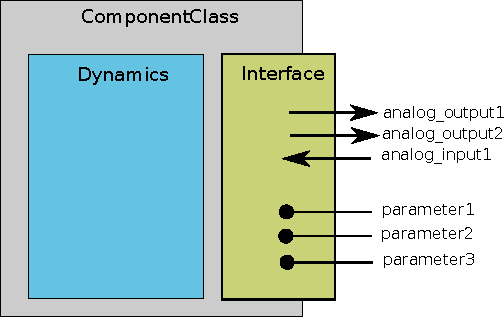
\includegraphics[width=8cm]{figures/component_simple.pdf}
\protect\caption{ComponentClass Overview (Simple)}
\label{fig:EX1_RegimeGraph}
\end{figure}

\subsubsection{Name attribute}
Each \ComponentClass requires a \textit{name} attribute. This name should be a valid identifier in the \href{http://msdn.microsoft.com/en-us/library/e7f8y25b.aspx}{ANSI C89 standard} and uniquely identify the {\ComponentClass} in current the scope.

\subsection{Parameter}
\label{sec:Parameter}

Parameters correspond to a placeholder for a numerical value with
dimension (this value can also be defined as dimensionless).

\begin{table}[H]
  \begin{edtable}{tabular}{llr}
    \toprule
    \multicolumn{3}{c}{\parbox{0.55\linewidth}{\center\textbf{Parameter Structure}}}\\
    \toprule
    \em{Attribute name} & \em{Type/Format} & \em{Required} \\
    \midrule
    name & \href{http://msdn.microsoft.com/en-us/library/e7f8y25b.aspx}{ANSI C89 identifier} & yes\\
    dimension & name:UnitDimension & yes\\
    \bottomrule
  \end{edtable}
\end{table}

It defines particular aspects of the model, such as the firing threshold,
reset voltage, the
decay time constant of a synapse model.  The instantiation of
Parameters at the Abstraction Layer level allow us to define the
dynamics of a general component.  It is then possible to instantiate
several variants of this component by attributing different values for
the {\Parameter}s, in the User Layer.  For example, if we are building
an integrate-and-fire neuron, we can specify that the Reset-Voltage
and the Firing-Threshold are parameters, write our dynamics in terms
of these parameters, then use the User Layer to provide parameters to
create different neurons. By definition, Parameters are set at the
start of the simulation, and remain constant throughout.


\subsubsection{Name attribute}
Each \Parameter requires a \textit{name} attribute. This name should be a valid identifier in the \href{http://msdn.microsoft.com/en-us/library/e7f8y25b.aspx}{ANSI C89 standard} and uniquely identify the {\Parameter} from all other elements in the \ComponentClass.

\subsubsection{Dimension attribute}
Each \Parameter requires a \textit{dimension} attribute. This attribute specifies the dimension of the units of the quantity that is expected to be passed to the \Parameter and should refer to the name of a \UnitDimension element in the global scope.


\subsection{AnalogSendPort}
\label{sec:AnalogSendPort}

{\AnalogSendPort}s of variables from the current component to be published externally to be read by other {\ComponentClass}es. Each {\AnalogSendPort} can be connected to multiple {\AnalogReceivePort}s and {\AnalogReducePort}s.

\begin{table}[H]
  \begin{edtable}{tabular}{llr}
    \toprule
    \multicolumn{3}{c}{\parbox{0.55\linewidth}{\center\textbf{AnalogSendPort Structure}}}\\
    \toprule
    \em{Attribute name} & \em{Type/Format} & \em{Required} \\
    \midrule
    name & \href{http://msdn.microsoft.com/en-us/library/e7f8y25b.aspx}{ANSI C89 identifier} & yes\\
    dimension & name:UnitDimension & yes\\
    \bottomrule
  \end{edtable}
\end{table}

\subsubsection{Name attribute}
Each \AnalogSendPort requires a \textit{name} attribute. This name should be a valid identifier in the \href{http://msdn.microsoft.com/en-us/library/e7f8y25b.aspx}{ANSI C89 standard} and uniquely identify the {\AnalogSendPort} from all other elements in the \ComponentClass.


\subsubsection{Dimension attribute}
Each \Parameter requires a \textit{dimension} attribute. This attribute specifies the dimension of the units of the quantity that is expected to be passed to the \Parameter and should refer to the name of a \UnitDimension element in the global scope.


\subsection{AnalogReceivePort}
\label{sec:AnalogReceivePort}

{\AnalogReceivePort}s allow variables that have been published externally to be used within the current component. Each \AnalogReceivePort can be connected to \emph{one} \AnalogSendPort.

\begin{table}[H]
  \begin{edtable}{tabular}{llr}
    \toprule
    \multicolumn{3}{c}{\parbox{0.55\linewidth}{\center\textbf{AnalogReceivePort Structure}}}\\
    \toprule
    \em{Attribute name} & \em{Type/Format} & \em{Required} \\
    \midrule
    name & \href{http://msdn.microsoft.com/en-us/library/e7f8y25b.aspx}{ANSI C89 identifier} & yes\\
    dimension & name:UnitDimension & yes\\
    \bottomrule
  \end{edtable}
\end{table}

\subsubsection{Name attribute}
Each \AnalogReceivePort requires a \textit{name} attribute. This name should be a valid identifier in the \href{http://msdn.microsoft.com/en-us/library/e7f8y25b.aspx}{ANSI C89 standard} and uniquely identify the {\AnalogReceivePort} from all other elements in the \ComponentClass.

\subsubsection{Dimension attribute}
Each \Parameter requires a \textit{dimension} attribute. This attribute specifies the dimension of the units of the quantity that is expected to be passed to the \Parameter and should refer to the name of a \UnitDimension element in the global scope.


\subsection{AnalogReducePort}
\label{sec:AnalogReducePort}

\begin{table}[H]
  \begin{edtable}{tabular}{llr}
    \toprule
    \multicolumn{3}{c}{\parbox{0.55\linewidth}{\center\textbf{AnalogReducePort Structure}}}\\
    \toprule
    \em{Attribute name} & \em{Type/Format} & \em{Required} \\
    \midrule
    name & \href{http://msdn.microsoft.com/en-us/library/e7f8y25b.aspx}{ANSI C89 identifier} & yes\\
    dimension & name:UnitDimension & yes\\
    operator & \lq\lq{}+\rq\rq{} | \lq\lq{}*\rq\rq{} & yes \\
    \bottomrule
  \end{edtable}
\end{table}



{\AnalogReducePort}s can receive data from any number of {\AnalogSendPort}s (including none). They
differ from \AnalogReceivePort in that they can be connected to multiple
{\AnalogSendPort}s. \AnalogReducePort take an additional operator,
{\tt reduce\_op}, which specifies how the data from multiple \AnalogSendPort
should be combined to produce a single value. Currently, the
only supported operations are \lq\lq{}$+$\rq\rq{} and \lq\lq{}$*$\rq\rq{}, which sum and multiply the inputs respectively.
The motivation for \AnalogReducePort is that it allows us to make our
\ComponentClass definitions more general. For example, if we are defining a
neuron, would define a \AnalogReducePort called \emph{InjectedCurrent}.
This allows us to write the membrane equation for that neuron as
$dV/dt = (1/C) * InjectedCurrents$.

Then, when we connect this neuron to synapses, current-clamps, etc, we
simply need to connect the SendPorts containing the currents of these
{\ComponentClass}es onto the \emph{InjectedCurrent} reduce-port, without having
to change our original \ComponentClass definitions.

\subsubsection{Name attribute}
Each \AnalogReducePort requires a \textit{name} attribute. This name should be a valid identifier in the \href{http://msdn.microsoft.com/en-us/library/e7f8y25b.aspx}{ANSI C89 standard} and uniquely identify the {\AnalogReducePort} from all other elements in the \ComponentClass.

\subsubsection{Dimension attribute}
Each \AnalogReducePort requires a \textit{dimension} attribute. This attribute specifies the dimension of the units of the quantity that is expected to be passed to the \AnalogReducePort and should refer to the name of a \UnitDimension element in the global scope.

\subsubsection{Operator attribute}
Each \AnalogReducePort requires a \textit{operator} attribute. The operator \lq\lq{}reduces\rq\rq{} the connected inputs to a single value at each time point. For example the following port,

\begin{lstlisting}
<AnalogReducePort name="total_membrane_current" dimension="current" operator="+"/>
\end{lstlisting}

will take all of the electrical currents that have been connected to it via {\AnalogSendPort}s and sum them together to get the total current passing through the membrane.


\subsection{EventSendPort}
\label{sec:EventSendPort}

\begin{table}[H]
  \begin{edtable}{tabular}{llr}
    \toprule
    \multicolumn{3}{c}{\parbox{0.55\linewidth}{\center\textbf{EventSendPort Structure}}}\\
    \toprule
    \em{Attribute name} & \em{Type/Format} & \em{Required} \\
    \midrule
    name & \href{http://msdn.microsoft.com/en-us/library/e7f8y25b.aspx}{ANSI C89 identifier} & yes\\
    \bottomrule
  \end{edtable}
\end{table}

\subsubsection{Name attribute}
Each \EventSendPort requires a \textit{name} attribute. This name should be a valid identifier in the \href{http://msdn.microsoft.com/en-us/library/e7f8y25b.aspx}{ANSI C89 standard} and uniquely identify the {\EventSendPort} from all other elements in the \ComponentClass.


\subsection{EventReceivePort}
\label{sec:EventReceivePort}

\begin{table}[H]
  \begin{edtable}{tabular}{llr}
    \toprule
    \multicolumn{3}{c}{\parbox{0.55\linewidth}{\center\textbf{EventReceivePort Structure}}}\\
    \toprule
    \em{Attribute name} & \em{Type/Format} & \em{Required} \\
    \midrule
    name & \href{http://msdn.microsoft.com/en-us/library/e7f8y25b.aspx}{ANSI C89 identifier} & yes\\
    \bottomrule
  \end{edtable}
\end{table}

\subsubsection{Name attribute}
Each \EventReceivePort requires a \textit{name} attribute. This name should be a valid identifier in the \href{http://msdn.microsoft.com/en-us/library/e7f8y25b.aspx}{ANSI C89 standard} and uniquely identify the {\EventReceivePort} from all other elements in the \ComponentClass.


\subsection{EventReducePort}
\label{sec:EventReducePort}
%
\begin{table}[H]
  \begin{edtable}{tabular}{llr}
    \toprule
    \multicolumn{3}{c}{\parbox{0.55\linewidth}{\center\textbf{EventReducePort Structure}}}\\
    \toprule
    \em{Attribute name} & \em{Type/Format} & \em{Required} \\
    \midrule
    name & \href{http://msdn.microsoft.com/en-us/library/e7f8y25b.aspx}{ANSI C89 identifier} & yes\\
    \bottomrule
  \end{edtable}
\end{table}

Event ports transmit discrete events. They are useful for example in
simulation of integrate-and-fire neurons to notify {\ComponentClass}es about neuron's
spiking. Event ports only have 2 modes:

\begin{itemize}
\item \AnalogSendPort - transmit events originating in this \ComponentClass which can be
read by
other {\ComponentClass}es
\item \AnalogReceivePort - receive events from another \ComponentClass \AnalogSendPort port.
Each recv port can be connected to \emph{multiple} \AnalogSendPort.
\end{itemize}

For example, a synapse component may have a \AnalogReceivePort connected to the
presynaptic neurons \AnalogSendPort port. When the presynaptic neuron fires;
it delivers an event to the synapse, which could cause it to produce current
flow in a post-synaptic neuron.


\subsubsection{Name attribute}
Each \EventReducePort requires a \textit{name} attribute. This name should be a valid identifier in the \href{http://msdn.microsoft.com/en-us/library/e7f8y25b.aspx}{ANSI C89 standard} and uniquely identify the {\EventReducePort} from all other elements in the \ComponentClass.


\subsection{Dynamics}
\label{sec:Dynamics}

\begin{table}[H]
  \begin{edtable}{tabular}{llr}
    \toprule
    \multicolumn{3}{c}{\parbox{0.55\linewidth}{\center\textbf{Dynamics Structure}}}\\
    \toprule
    \em{Element type} & \em{Multiplicity} & \em{Required} \\
    \midrule
    \StateVariable & set & no \\ 
    \Regime & set & yes\\
    \Alias & set & no\\
    \bottomrule
  \end{edtable}
\end{table}

The \Dynamics block represents the \emph{internal} mechanisms
governing the behaviour of the component.  For most of the models
these dynamics are non-linear, presenting transitions between
different regimes at particular values of one or different {\StateVariable}s.
To create a representation that include both simple
dynamics and non-linear dynamics, the \Dynamics block can contains the
following concepts:

\begin{itemize}
\item \StateVariable (section~\ref{state-var})
\item \Regime (section~\ref{regime}) that describe the dynamics of the
system for a particular domain of \StateVariable
\item \Transition (section~\ref{transition}) that links two
regimes: the Source \Regime and the Target \Regime, and can be triggered by
an event or a condition. If a component is in the Source \Regime, and the
transition is triggered, then the component moves into the Target \Regime.
\item \Alias (section~\ref{alias})
\end{itemize}


These different concepts are the building blocks of a graph, called
the {\tt Regime Graph} (illustrated in Figure~\ref{SimpleRegimeGraph}),
where the \Regime forms the vertices and the \Transition form the
directional edges of the {\tt Regime Graph}. This graph must have at
least one \Regime, and contain no regime islands. At any given time,
a component will be in a single \Regime, and can change which \Regime
it is in through \Transition.

\begin{figure}[htb!]
\center
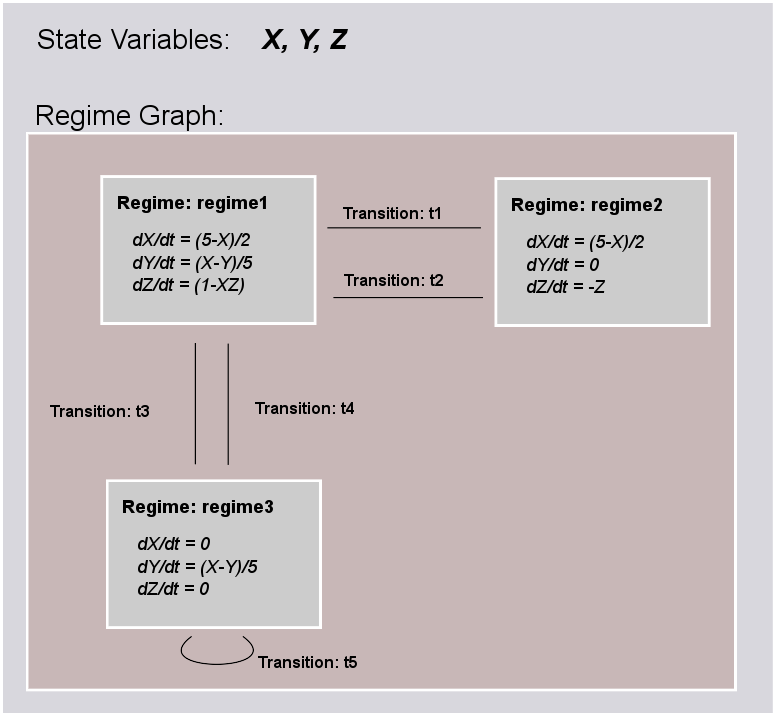
\includegraphics[width=14cm]{images/SimpleRegimeGraph.png}
\protect\caption{The dynamics block for an example component.}
\label{SimpleRegimeGraph}
\end{figure}

An example dynamics in Figure~\ref{SimpleRegimeGraph} has three {\StateVariable}s,
\emph{X,Y} and \emph{Z}, and a state graph with three {\Regime}s, \emph{regime1},
\emph{regime2} and \emph{regime3}. At any time, a component will be in one of
these regimes, and the state variables will evolve accordingly.

\subsection{StateVariable}
\label{sec:StateVariable}

\begin{table}[H]
  \begin{edtable}{tabular}{llr}
    \toprule
    \multicolumn{3}{c}{\parbox{0.55\linewidth}{\center\textbf{StateVariable Structure}}}\\
    \toprule
    \em{Attribute name} & \em{Type/Format} & \em{Required} \\
    \midrule
    name & \href{http://msdn.microsoft.com/en-us/library/e7f8y25b.aspx}{ANSI C89 identifier} & yes\\
    dimension & name:UnitDimension & yes\\
    \bottomrule
  \end{edtable}
\end{table}

The internal state of a component is defined by a set of \StateVariable
-- variables that can change either continuously or discontinuously as a
function of time.

The \StateVariable changes happen in two ways:
\begin{quote}
\begin{itemize}
\item continuously through \textbf{TimeDerivatives} (in {\Regime}s),
which define the {\StateVariable}s evolution over time, for example
$dX/dt=1-X$.
\item discretely through \StateAssignment (in \Transition),
which make discrete changes to a \StateVariable value, for example
$X = X + 1$.
\end{itemize}
\end{quote}

\subsubsection{Name attribute}
Each \StateVariable requires a \textit{name} attribute. This name should be a valid identifier in the \href{http://msdn.microsoft.com/en-us/library/e7f8y25b.aspx}{ANSI C89 standard} and uniquely identify the {\StateVariable} from all other elements in the \ComponentClass.

\subsubsection{Dimension attribute}
Each \StateVariable requires a \textit{dimension} attribute. This attribute specifies the dimension of the units of the quantities that \StateVariable is expected to be initialised and updated with and should refer to the name of a \UnitDimension element in the global scope.


\subsection{Regime}
\label{sec:Regime}

\begin{table}[H]
  \begin{edtable}{tabular}{llr}
    \toprule
    \multicolumn{3}{c}{\parbox{0.55\linewidth}{\center\textbf{Regime Structure}}}\\
    \toprule
    \em{Attribute name} & \em{Type/Format} & \em{Required} \\
    \midrule
    name & \href{http://msdn.microsoft.com/en-us/library/e7f8y25b.aspx}{ANSI C89 identifier} & yes\\
    \midrule
    \em{Element type} & \em{Multiplicity} & \em{Required} \\
    \midrule
    \TimeDerivative & set & no \\ 
    \OnCondition & set & no\\
    \OnEvent & set & no\\
    \bottomrule
  \end{edtable}
\end{table}

A \Regime is defined in NineML as a system of ODEs in time
on \StateVariable.  As such, \Regime defines how the {\StateVariable}s
change (propagate in time) between subsequent {\Transition}s. \Regime is
defined to have non-vanishing temporal extent. Once construction of
the \Regime is complete, it should have defined the following
properties:

\begin{itemize}
\item An unordered collection of {\StateVariable}s which are
propagated when the {\Regime} is active.
\item a set of \TimeDerivative, one for each \StateVariable
of the \ComponentClass, which define how the \StateVariable
evolve over time in the form $\frac{dx_{i}}{dt} = f(x\_0, ..., x\_i, t)$.
\item The independent variable must be shared between the collection
of {\StateVariable}s and their propagators in a \Regime.
\end{itemize}

\note{If a {\TimeDerivative} for a \StateVariable is not defined
in a \Regime, it is assumed to be zero.}

It is important to note that, at the current stage of development, we are only
considering "Temporal regimes". In the future, the concept could be extended
to more general cases where the independent variable can be anything (space
for example)

\subsubsection{Name attribute}
Each \Regime requires a \textit{name} attribute. This name should be a valid identifier in the \href{http://msdn.microsoft.com/en-us/library/e7f8y25b.aspx}{ANSI C89 standard} and uniquely identify the {\Regime} from all other elements in the \ComponentClass.


\subsection{TimeDerivative}
\label{sec:TimeDerivative}

\begin{table}[H]
  \begin{edtable}{tabular}{llr}
    \toprule
    \multicolumn{3}{c}{\parbox{0.55\linewidth}{\center\textbf{TimeDerivative Structure}}}\\
    \toprule
    \em{Attribute name} & \em{Type/Format} & \em{Required} \\
    \midrule
    variable & name:StateVariable & yes\\
    \midrule
    \em{Element type} & \em{Multiplicity} & \em{Required} \\
    \midrule
    \MathInline & singleton & yes \\ 
    \bottomrule
  \end{edtable}
\end{table}

\subsubsection{Variable attribute}
Each \TimeDerivative requires a \textit{variable} attribute. This should refer to the name of a \StateVariable in the \ComponentClass. Only one \TimeDerivative is allow per \textit{variable} in each \Regime.


\subsection{OnEvent}
\label{sec:OnEvent}

An OnEvent block is activated when the dynamics component receives an event from published from an external component.

\vspace*{-0.25ex}
\begin{table}[H]
  \begin{edtable}{tabular}{llr}
    \toprule
    \multicolumn{3}{c}{\parbox{0.55\linewidth}{\center\textbf{OnEvent Structure}}}\\
    \toprule
    \em{Attribute name} & \em{Type/Format} & \em{Required} \\
    \midrule
    port & name:EventReceivePort | name:EventReducePort & yes\\
    \midrule
    \em{Element type} & \em{Multiplicity} & \em{Required} \\
    \midrule
    \Transition & singleton & no \\    
    \StateAssignment & set & no\\
    \EventOut & set & no\\
    \bottomrule
  \end{edtable}
\end{table}

\subsubsection{Port attribute}
Each \OnEvent requires a \textit{port} attribute. This should refer to the name of an \EventReceivePort or an \EventReducePort in the \ComponentClass interface.


\subsection{OnCondition}
\label{sec:OnCondition}

An OnCondition block is activated when the condition in the \Trigger block is met.

\begin{table}[H]
  \begin{edtable}{tabular}{llr}
    \toprule
    \multicolumn{3}{c}{\parbox{0.55\linewidth}{\center\textbf{OnCondition Structure}}}\\
    \toprule
    \em{Element type} & \em{Multiplicity} & \em{Required} \\
    \midrule
    \Trigger & singleton & yes \\
    \Transition & singleton & no \\
    \StateAssignment & set & no\\
    \EventOut & set & no\\
    \bottomrule
  \end{edtable}
\end{table}

{\OnCondition}s are the mathematical expressions which define
when a {\Transition} should be triggered.
{\OnCondition}s are any arbitrary combination of \emph{Logical
Operations} (and, or, noop, etc.) on the
result of any arbitrary combination of \emph{Relational Operations}
($>$,$<$,$==$,$<=$,$>=$, etc.) on
{\StateVariable}s. At any given time in the {\Regime},
the {\OnCondition} expression then evaluates to True or False
{\tt Boolean} result. For example, the following are valid
{\OnCondition}s

\begin{lstlisting}
x>10
x>10 & y<20
x>exp(-cos(y)) | y<sin(t)+5
x==15
\end{lstlisting}

A {\OnCondition} which persistently evaluates to True violates
the definition that {\Transition}s should have vanishing
temporal extent, and the behaviour for this case is undefined, but it
would be preferable for the implementation to produce an error message
to the user.


\subsection{Trigger}
\label{sec:Trigger}

The trigger block defines the condition on which the \OnCondition block is activiated.

\begin{table}[H]
  \begin{edtable}{tabular}{llr}
    \toprule
    \multicolumn{3}{c}{\parbox{0.55\linewidth}{\center\textbf{Trigger Structure}}}\\
    \toprule
    \em{Element type} & \em{Multiplicity} & \em{Required} \\
    \midrule
    \MathInline & singleton & yes \\ 
    \bottomrule
  \end{edtable}
\end{table}



\subsection{Transition}
\label{sec:Transition}

{\Transition}s define the transition between \Regime blocks.

\begin{table}[H]
  \begin{edtable}{tabular}{llr}
    \toprule
    \multicolumn{3}{c}{\parbox{0.55\linewidth}{\center\textbf{Transition Structure}}}\\
    \toprule
    \em{Attribute name} & \em{Type/Format} & \em{Required} \\
    \midrule
    to & name:Regime & yes\\
    \bottomrule
  \end{edtable}
\end{table}

Movement between several instances of \Regime happens via \Transition.
A {\Transition} is defined in NineML as having
a source and target {\Regime}, where the target
{\Regime} can be the same as the source (For example \emph{t5}
in Figure~\ref{SimpleRegimeGraph}). There are two types of \Transition:

\begin{itemize}
\item An \OnCondition function of the \StateVariable, for
example $X > Y$.
\item An \OnEvent on an input from an \EventReceivePort. (See section~\ref{port}).
\end{itemize}

During either type of transition three things can happen:
\begin{itemize}
\item The component can change regime. For example, in figure 2, if
the component is in \emph{regime3}, and the trigger for \emph{t3} is
satisfied, then the component will move into \emph{regime1}.
\item \textbf{StateAssignment}s can take place, for example, $X=0$
\item The component can send \EventOut
\end{itemize}

During a transition, multiple \StateAssignment and \EventOut can occur.
(For more on the resolution of {\Transition}s see Appendix
section~\ref{resolution})

{\Transition}s have a vanishing temporal extent (i.e. they are
event-like). Once construction of a {\Transition} is complete, it
should have defined the following properties:
\begin{itemize}
\item The {\OnCondition} or {\EventReceivePort} which
triggers the {\Transition}
\item A set of \StateAssignment and \EventOut objects
\item The label of the source {\Regime}, and the label of the target
{\Regime}, which may be the same as the source {\Regime}.
\end{itemize}

\subsubsection{To attribute}
Each \Transition requires a \textit{to} attribute. This should refer to the name of a \Regime element in the \ComponentClass.


\subsection{StateAssignment}
\label{sec:StateAssignment}

\begin{table}[H]
  \begin{edtable}{tabular}{llr}
    \toprule
    \multicolumn{3}{c}{\parbox{0.55\linewidth}{\center\textbf{StateAssignment Structure}}}\\
    \toprule
    \em{Attribute name} & \em{Type/Format} & \em{Required} \\
    \midrule
    variable & name:StateVariable & yes\\
    \midrule
    \em{Element type} & \em{Multiplicity} & \em{Required} \\
    \midrule
    \MathInline & singleton & yes \\     
    \bottomrule
  \end{edtable}
\end{table}

\subsubsection{Variable attribute}
Each \StateAssignment requires a \textit{variable} attribute. This should refer to the name of a \StateVariable in the \ComponentClass. Only one \StateAssignment is allow per \textit{variable} in each \OnEvent or \OnCondition block.



\subsection{EventOut}
\label{sec:EventOut}

\begin{table}[H]
  \begin{edtable}{tabular}{llr}
    \toprule
    \multicolumn{3}{c}{\parbox{0.55\linewidth}{\center\textbf{EventOut Structure}}}\\
    \toprule
    \em{Attribute name} & \em{Type/Format} & \em{Required} \\
    \midrule
    port & name:EventSendPort & yes\\
    \bottomrule
  \end{edtable}
\end{table}

\subsubsection{Port attribute}
Each \OnEvent requires a \textit{port} attribute. This should refer to the name of an \EventSendPort in the \ComponentClass interface.

\subsection{Alias}
\label{sec:Alias}


\begin{table}[H]
  \begin{edtable}{tabular}{llr}
    \toprule
    \multicolumn{3}{c}{\parbox{0.55\linewidth}{\center\textbf{Alias Structure}}}\\
    \toprule
    \em{Attribute name} & \em{Type/Format} & \em{Required} \\
    \midrule
    name & \href{http://msdn.microsoft.com/en-us/library/e7f8y25b.aspx}{ANSI C89 identifier} & yes\\
    \midrule
    \em{Element type} & \em{Multiplicity} & \em{Required} \\
    \midrule
    \MathInline & singleton & yes \\ 
    \bottomrule
  \end{edtable}
\end{table}

\note{\Alias is defined in the Dynamics, \emph{not} in the
\Regime. This means that aliases are the same across all regimes.}

An alias corresponds to an intermediate variable allowing to store an
information and to reuse it at different places in the definition of
the dynamics.

\textbf{Aliases} are motivated from two problems:

\begin{itemize}
\item {\bf substitution}: rather than writing long expressions for functions of
\StateVariable, we can define an \Alias once. For example, we can define chains
of {\Alias}es:
%
\begin{lstlisting}
m_alpha = (alphaA+alphaB*V)/(alphaC+exp((alphaD+V/alphaE)))
m_beta = (betaA+betaB*V)/(betaC+exp((betaD+V/betaE)))
minf = m_alpha/(m_alpha+m_beta)
mtau = 1./(m_alpha+m_beta)
dm/dt = (1/C)*(minf-m)/mtau
\end{lstlisting}

In this case, $m_{alpha}$, $m_{beta}$, $minf$ and $mtau$ are all
alias definitions. There is no reason we couldn't expand our $dm/dt$
description out to eliminate these intermediate {\Alias}es, but the expression
would be very long and difficult to read.

\item {\bf Accessing intermediate variable}: if we would like to communicate a
value other than a simple \StateVariable to another \ComponentClass. For
example, if we have a component representing a
neuron, which has an internal \StateVariable, 'V', we may be interested in
transmitting a current, for example $i=g*(E-V)$.

\end{itemize}


\subsubsection{Name attribute}
Each \Alias requires a \textit{name} attribute. This name should be a valid identifier in the \href{http://msdn.microsoft.com/en-us/library/e7f8y25b.aspx}{ANSI C89 standard} and uniquely identify the {\Alias} from all other elements in the \ComponentClass.


\subsection{MathInline}
\label{sec:MathInline}

\begin{table}[H]
  \begin{edtable}{tabular}{lr}
    \toprule
    \multicolumn{2}{c}{\parbox{0.55\linewidth}{\center\textbf{MathInline Structure}}}\\
    \toprule
    \em{Description of text} & \em{Required} \\
    \midrule
    maths-expression & yes\\
    \bottomrule
  \end{edtable}
\end{table}


A block used to specify mathematical expressions. The expression is expected to
be in \texttt{C} style and given as text. MathML support is planned in future versions of NineML

Depending on the context; MathInline blocks should return an expression that
evaluates to either a \verb|Boolean| (when used as the trigger for
{\OnCondition}s) or a \verb|floating-point| number ( when used  as a
right-hand-side for  {\Alias}es, {\TimeDerivative}s \& {\StateAssignment}s).

The following operators are supported, with the same precedence levels as ANSI
C89. All
numbers/variables are assumed to be \verb|floating-point| numbers, not integers.

\begin{itemize}
\item Arithmetic operators
\begin{itemize}
\item Addition \verb|+|
\item Subtraction \verb|-|
\item Division \verb|/|
\item Multiplication \verb|*|
\end{itemize}

\item Relational operators
\begin{itemize}
\item Greater than \verb|>|
\item Greater than equal \verb|>=|
\item Lesser than \verb|<|
\item Lesser than equal \verb|<=|
\end{itemize}

Logical operators
\begin{itemize}
\item Logical And: \verb|&&|
\item Logical Or:  \verb+||+
\item Logical Not: \verb|!|
\end{itemize}

\end{itemize}

The following symbols are built in, and cannot be redefined:
\begin{itemize}
\item pi
\item e
\end{itemize}


The following functions are built in, and cannot be redefined:
\begin{itemize}
\item \verb|exp(x)|
\item \verb|sin(x)|
\item \verb|cos(x)|
\item \verb|log(x)|
\item \verb|log10(x)|
\item \verb|pow(x)|
\item \verb|sinh(x)|
\item \verb|cosh(x)|
\item \verb|tanh(x)|
\item \verb|sqrt(x)|
\item \verb|atan(x)|
\item \verb|asin(x)|
\item \verb|acos(x)|
\item \verb|asinh(x)|
\item \verb|acosh(x)|
\item \verb|atanh(x)|
\item \verb|atan2(x)|
\item \verb|ceil(x)|
\item \verb|floor(x)|
\end{itemize}

These functions take the same parameters and are defined as per ANSI C89.

The following random distributions are available, through the \verb|random|
namespace,
although their use is only allowed within \StateAssignment blocks:

\begin{itemize}
\item \verb|random.uniform|
\item \verb|random.normal|
\item \verb|random.binomial(N,P)|
\item \verb|random.poisson(L)|
\item \verb|random.exponential(L)|
\end{itemize}


\subsection{RandomDistribution}
\label{sec:RandomDistribution}

\begin{table}[H]
  \begin{edtable}{tabular}{llr}
    \toprule
    \multicolumn{3}{c}{\parbox{0.55\linewidth}{\center\textbf{ConnectionRule Structure}}}\\
    \toprule
    \em{Element type} & \em{Multiplicity} & \em{Required} \\
    \midrule
    \BuiltInDistribution & singleton & yes\\
    \bottomrule
  \end{edtable}
\end{table}

\subsection{BuiltInDistribution}
\label{sec:BuiltInDistribution}


\begin{table}[H]
  \begin{edtable}{tabular}{llr}
    \toprule
    \multicolumn{3}{c}{\parbox{0.55\linewidth}{\center\textbf{ProbabilisticConnectivity Structure}}}\\
    \toprule
    \em{Attribute name} & \em{Type/Format} & \em{Required} \\
    \midrule
    uncertml &  \href{http://en.wikipedia.org/wiki/Uniform_resource_locator}{URL}  & yes\\
    \bottomrule
  \end{edtable}
\end{table}


\subsection{ConnectionRule}
\label{sec:ConnectionRule}

\begin{table}[H]
  \begin{edtable}{tabular}{llr}
    \toprule
    \multicolumn{3}{c}{\parbox{0.55\linewidth}{\center\textbf{ConnectionRule Structure}}}\\
    \toprule
    \em{Element type} & \em{Multiplicity} & \em{Required} \\
    \midrule
    \AllToAll | \OneToOne | \ProbabilisticConnectivity | \ExplicitConnectionList & singleton & yes\\
    \bottomrule
  \end{edtable}
\end{table}

In Version 1.0 of the NineML standard, connection rules must be one of four built-in types, \AllToAll, \OneToOne, \ProbabilisticConnectivity or \ExplicitConnectionList. In future versions, extensions 
are planned to this framework to allow richer connectivity rules.

\subsection{AllToAll}
\label{sec:AllToAll}

All cells in the source population are connected to all cells in the destination population.

\note{\AllToAll has no attributes or child-elements}

\subsection{OneToOne}
\label{sec:OneToOne}

Each cell in the source population is connected to the cell in the destination population with the corresponding index. Note that this requires that the source and destination populations be the same size.

\note{\OneToOne has no attributes or child-elements}

\subsection{ProbabilisticConnectivity}
\label{sec:ProbabilisticConnectivity}

\begin{table}[H]
  \begin{edtable}{tabular}{llr}
    \toprule
    \multicolumn{3}{c}{\parbox{0.55\linewidth}{\center\textbf{ProbabilisticConnectivity Structure}}}\\
    \toprule
    \em{Attribute name} & \em{Type/Format} & \em{Required} \\
    \midrule
    probability & name:Parameter & yes\\
    \bottomrule
  \end{edtable}
\end{table}

All cells in the source population are connected to cells in the destination population with a probability defined by the \ConnectionProbability element.

\subsubsection{Probability attribute}

Each \ProbabilisticConnectivity element requires a \textit{probability} attribute. This attribute should refer to a name of a dimensionless \Parameter in the enclosing \ComponentClass. The properties supplied to this parameter should either be a dimensionless \HomogeneousValue representing the probability of a connection between all source and destination cell pairs, or a \ValueList or \ExternalValueList of size $M{\times}N$, where $M$ and $N$ are the size of the source and destination populations respectively. In the case of the \ValueList or \ExternalValueList properties, the list represents probabilities of connections existing between the first cell in the source population with every cell in the destination population in order of their index, followed by the second cell in the source with with every cell in the destination population in order of their index and so forth for each cell in the source population.

\subsection{ExplicitConnectionList}
\label{sec:ExplicitConnectionList}

\begin{table}[H]
  \begin{edtable}{tabular}{llr}
    \toprule
    \multicolumn{3}{c}{\parbox{0.55\linewidth}{\center\textbf{ProbabilisticConnectivity Structure}}}\\
    \toprule
    \em{Attribute name} & \em{Type/Format} & \em{Required} \\
    \midrule
    source-indices & name:Parameter & yes\\
    target-indices & name:Parameter & yes\\
    \bottomrule
  \end{edtable}
\end{table}

Cells in the source population are connected to cells in the destination population as specified by an explicit lists.

\subsubsection{Source-indices attribute}

Each \ExplicitConnectionList element requires a \textit{source-indices} attribute. This attribute should refer to a name of a dimensionless \Parameter in the enclosing \ComponentClass. The properties supplied to this parameter should be a \ValueList or \ExternalValueList drawn from the set $\{1,\ldots,M\}$ where $M$ is the size of the source population and be the same length as the property supplied to the \textit{target-indices} parameter.

\subsubsection{Target-indices attribute}

Each \ExplicitConnectionList element requires a \textit{target-indices} attribute. This attribute should refer to a name of a dimensionless \Parameter in the enclosing \ComponentClass. The properties supplied to this parameter should be a \ValueList or \ExternalValueList drawn from the set $\{1,\ldots,N\}$ where $N$ is the size of the source population and be the same length as the property supplied to the \textit{source-indices} parameter.

\newpage

\section{User Layer}
\label{UserL}

\subsection{Component}
\label{sec:Component}

\begin{table}[H]
  \begin{edtable}{tabular}{llr}
    \toprule
    \multicolumn{3}{c}{\parbox{0.55\linewidth}{\center\textbf{Component Structure}}}\\
    \toprule
    \em{Attribute name} & \em{Type/Format} & \em{Required} \\
    \midrule
    name & \href{http://msdn.microsoft.com/en-us/library/e7f8y25b.aspx}{ANSI C89 identifier} & yes\\
    \midrule
    \em{Element type} & \em{Multiplicity} & \em{Required} \\
    \midrule
    \Definition | \Prototype & singleton & yes \\ 
    \Property & set & no\\
    \bottomrule
  \end{edtable}
\end{table}

The basic building block of NineML User Layer is called component. In the
User Layer description component is a reference to a \ComponentClass
object defined in the Abstraction Layer. Abstraction Layer defines the
mathematics of the component and this definition is then referred in the
User Layer through an object of type \Definition.

In addition to the \Definition object, the component encapsulates
user-given ID or label, and a set of \Property objects. The composition
of this set of properties is defined in the Abstraction Layer (or externally)
and instantiated in the User Layer description of component. The mapping
between mathematical description of the object in the abstraction
layer and the corresponding properties labels in the User Layer are
provided in this specification.

User can add a note to a component. These notes are intended to provide
a specific reference to the research paper page where this component is
described and similar kind of information. These notes are not intended
to duplicate the Abstraction Layer documentation or any other
documentation, thus they shall not provide mathematical description and
other details of the component implementation. Note can contain text
(type {\tt String}) or link to an Internet resource (type {\tt URL}).

To reduce the size of the resulting model description user can refer to
already described component by referencing their label instead of providing
a link to the Abstraction Layer or external definition. In this case the
properties of the component that have to be redefined are stated explicitly,
the properties that are inherited from the original description are omitted.

If the simulator only supports User Layer, then the simulator developers
can create mappings directly between the reference to a definition in the
User Layer description of the component and the intrinsic simulator code
that implements the same mathematics.

\subsubsection{Name attribute}
Each \Component requires a \textit{name} attribute. This name should be a valid identifier in the \href{http://msdn.microsoft.com/en-us/library/e7f8y25b.aspx}{ANSI C89 standard} and uniquely identify the {\Component} from all other elements in the global scope.

\subsection{Definition}
\label{sec:Definition}

\begin{table}[H]
  \begin{edtable}{tabular}{llr}
    \toprule
    \multicolumn{3}{c}{\parbox{0.55\linewidth}{\center\textbf{Definition Structure}}}\\
    \toprule
    \em{Attribute name} & \em{Type/Format} & \em{Required} \\
    \midrule
    url & \href{http://en.wikipedia.org/wiki/Uniform_resource_locator}{URL} & no\\
    \midrule
    \em{Text format} & \; & \em{Required} \\
    \midrule
    name:ComponentClass & \; & no \\ 
    \bottomrule
  \end{edtable}
\end{table}

All constructs in the User Layer have their mathematical or algorithmical
definitions in the Abstraction Layer. Definition is an object that
establishes a link between User Layer component and Abstraction Layer
\ComponentClass. This \ComponentClass can be located either internal to the current
file or externally as specified by the \textit{url} attribute.

\subsubsection{Url attribute}
If the \ComponentClass referenced by the definition element is defined outside the current file, the \textit{url} attribute specifies a \href{http://en.wikipedia.org/wiki/Uniform_resource_locator}{Uniform Resource Locator (URL)} for the file which contains the \ComponentClass definition.

\subsubsection{Text}
\draftnote{I know we discussed this but I still am not sure it is a good idea to be able to drop the \ComponentClass name if it is the only \ComponentClass in the file. Because if someone adds a second \ComponentClass to the file it will break any (potentially remote) references to it}
If the referenced \ComponentClass is in the current file or there is more than one \ComponentClass in the file located by the \textit{url} attribute, the name of the \ComponentClass needs to be provided in the text of \Definition element.

\subsection{Prototype}
\label{sec:Prototype}

\begin{table}[H]
  \begin{edtable}{tabular}{llr}
    \toprule
    \multicolumn{3}{c}{\parbox{0.55\linewidth}{\center\textbf{Prototype Structure}}}\\
    \toprule
    \em{Attribute name} & \em{Type/Format} & \em{Required} \\
    \midrule
    url & \href{http://en.wikipedia.org/wiki/Uniform_resource_locator}{URL} & yes\\
    \midrule
    \em{Text format} & \; & \em{Required} \\
    \midrule
    name:Component & \; & no \\ 
    \bottomrule
  \end{edtable}
\end{table}

\Prototype is a User Layer object that can replace \Definition object
in situations where user needs to reuse the same definition for multiple
instances of objects. In this case the first instance shall be described using
\Definition and the rest can use the first one through \Reference.
Label in the \Reference must match a label in a previously defined
component.

\subsubsection{Url attribute}
If the prototype \Component is defined outside the current file, the \textit{URL} attribute specifies a \href{http://en.wikipedia.org/wiki/Uniform_resource_locator}{Uniform Resource Locator (URL)} for the file which contains the prototype \Component.

\subsubsection{Text}
If the prototype \Component is in the current file or there is more than one \Component in the file located by the \textit{url} attribute, the name of the prototype \Component needs to be provided in the text of \Prototype element.

\subsection{Property}
\label{sec:Property}

\begin{table}[H]
  \begin{edtable}{tabular}{llr}
    \toprule
    \multicolumn{3}{c}{\parbox{0.55\linewidth}{\center\textbf{Property Structure}}}\\
    \toprule
    \em{Attribute name} & \em{Type/Format} & \em{Required} \\
    \midrule
    name & name:Parameter & yes\\
    \midrule
    \em{Element type} & \em{Multiplicity} & \em{Required} \\
    \midrule
    \Quantity & singleton & yes \\ 
    \bottomrule
  \end{edtable}
\end{table}


Property is a User Layer object that instantiates values in simple
Abstraction Layer \Parameter and combines described in the quantity object
and a label. The label should match the corresponding label in the
Abstraction Layer \Parameter definition.

The user can set the value of the property and (when applicable for the data
type, e.g. \Quantity) the units of measurement. These units are also
checked against the dimensionality of the corresponding property definition
in the Abstraction Layer.

\subsubsection{Name attribute}
Each \Property requires a \textit{name} attribute. This should refer to the name of a \Parameter in the corresponding \ComponentClass of the \Component.

\subsection{Quantity}
\label{sec:Quantity}

Quantity is a compound data type object that encapsulates a numerical value
and a unit of measurements. Unit has to be of one of the \Units type.
Any numeric quantity in the language (except counters) has to be of this type,
dimensionless quantities shall use predefined empty \Units.
\draftnote{I have moved the \Component->\RandomDistribution outside of the a \lq\lq{}RandomDistribution\rq\rq{}
element here, partly because then we would need to come up with a different name for it, and partly as it doesn\rq{}t seem necessary}
\begin{table}[H]
  \begin{edtable}{tabular}{llr}
    \toprule
    \multicolumn{3}{c}{\parbox{0.55\linewidth}{\center\textbf{Quantity Structure}}}\\
    \toprule
    \em{Attribute name} & \em{Type/Format} & \em{Required} \\
    \midrule
    units & name:Units & no\\
    \midrule
    \em{Element type} & \em{Multiplicity} & \em{Required} \\
    \midrule
    \HomogeneousValue | \Component->\RandomDistribution | \ValueList | \ExternalValueList & singleton & yes \\
    \bottomrule
  \end{edtable}
\end{table}

There are two kinds of quantities: values of the first kind are given to the
model by the user and stay fixed, values of a second kind are computed within
the model during simulation. For all practical reasons the syntax of the user
layer descriptions is identical for both kinds of quantities. Furthermore,
because NineML does not provide any default values for quantities, it is a
job of the user to provide initial values for all defined quantities. To
ensure the integrity of the model NineML requires all initial values to be
set in the User Layer description. For batch simulations and other
modifications any of the values given in the User Layer can be overwritten
by a simulation setup description, but this is outside of the scope of the
current version of NineML.

Some quantities can have values drawn from random distribution. In
this case User Layer description of the quantities includes a
reference to a random distribution component instead of a numeric
value.  Other quantities might be calculated according to some
function dependent on some other quantities. These can be defined
through the type Functionby including inline Abstraction Layer
definitions or MathML.

\subsubsection{Units attribute}
The \textit{units} attribute specifies the units of the quantity and should refer to the name of a \Units element in the global scope. If it is omitted then the quantity is considered to be dimensionless.


\subsection{HomogeneousValue}
\label{sec:HomogeneousValue}

\draftnote{Instead of \lq\lq{}SingleValue\rq\rq{}, I thought \HomogeneousValue was a better name for this, thoughts?}
\begin{table}[H]
  \begin{edtable}{tabular}{llr}
    \toprule
    \multicolumn{3}{c}{\parbox{0.55\linewidth}{\center\textbf{HomogeneousValue Structure}}}\\
    \toprule
    \em{Text format} & \; & \em{Required} \\
    \midrule
    numeric value & \; & yes \\ 
    \bottomrule
  \end{edtable}
\end{table}

\subsection{ValueList}
\label{sec:ValueList}

\draftnote{I thought that \ValueList and \ValueListRow would be sufficient to provide the XML version explicit lists for demonstration purposes}

\begin{table}[H]
  \begin{edtable}{tabular}{llr}
    \toprule
    \multicolumn{3}{c}{\parbox{0.55\linewidth}{\center\textbf{ValueList Structure}}}\\
    \toprule
    \em{Element type} & \em{Multiplicity} & \em{Required} \\
    \midrule
    \ValueListRow & set & no \\
    \bottomrule
  \end{edtable}
\end{table}

\subsection{ValueListRow}
\label{sec:ValueListRow}

\begin{table}[H]
  \begin{edtable}{tabular}{llr}
    \toprule
    \multicolumn{3}{c}{\parbox{0.55\linewidth}{\center\textbf{ValueListRow Structure}}}\\
    \toprule
    \em{Attribute name} & \em{Type/Format} & \em{Required} \\
    \midrule
    index & integer & yes \\
    \midrule
    \em{Text format} & \; & \em{Required} \\
    \midrule
    numeric value & \; & yes\\
    \bottomrule
  \end{edtable}
\end{table}

\subsubsection{Index attribute}
The \textit{index} attribute specifies the index of the \ValueListRow in the \ValueList.

\note{This preserves the non-order specific nature of elements in NineML}

\subsection{ExternalValueList}
\label{sec:ExternalValueList}

\draftnote{This name is different to what we discussed in the meeting, do you like it?}

\begin{table}[H]
  \begin{edtable}{tabular}{llr}
    \toprule
    \multicolumn{3}{c}{\parbox{0.55\linewidth}{\center\textbf{ExternalValueList Structure}}}\\
    \toprule
    \em{Attribute name} & \em{Type/Format} & \em{Required} \\
    \midrule
    url & \href{http://en.wikipedia.org/wiki/Uniform_resource_locator}{URL} & yes\\
    mimetype & \href{http://en.wikipedia.org/wiki/Internet_media_type}{MIME type}  & yes\\
    column-name & name:data-column & no\\    
    \bottomrule
  \end{edtable}
\end{table}

\subsubsection{Url attribute}
The \textit{url} attribute specifies a \href{http://en.wikipedia.org/wiki/Uniform_resource_locator}{Uniform Resource Locator (URL)} for the external data file.

\subsubsection{Mimetype attribute}
The \textit{mimetype} attribute specifies the data format for the external value list. Currently, only two formats are supported \lstinline|application/vnd.nineml.valuelist.text| and \lstinline|application/vnd.nineml.valuelist.hdf5|. 

\draftnote{What do you think of these descriptions? I am a bit hazy on the structure of HDF5 could someone clean up my description?}
\begin{itemize}
\item \lstinline|application/vnd.nineml.valuelist.text| - an ASCII text file with a single row of white-space separated column names, followed by arbitrarily many white-space separated data rows of numeric values. Each numeric value is associated with the column name of the same column index and therefore the number of items in each row must be the same.
\item \lstinline|application/vnd.nineml.valuelist.hdf5| - a \href{http://www.hdfgroup.org/HDF5/}{HDF5} data file containing a single level of named members of array->float type.
\end{itemize}
\tracingall

\subsubsection{Column-name attribute}
\draftnote{Again, should we require column names to be provided to avoid problems if second columns are added later?}
If there is more than one data column in the external file then the \textit{column-name} attribute must be provided to specify which column is referenced.

\subsection{Population}
\label{sec:Population}

Population elements define sets of neuron components of the same class. The size of the set is specified by the {\tt number} attribute. The properties of the neuron components can be constant across the population, randomly distributed, individually specified or as a function of neuron index.  


\begin{table}[H]
  \begin{edtable}{tabular}{llr}
    \toprule
    \multicolumn{3}{c}{\parbox{0.55\linewidth}{\center\textbf{Population Structure}}}\\
    \toprule
    \em{Attribute name} & \em{Type/Format} & \em{Required} \\
    \midrule
    name & \href{http://msdn.microsoft.com/en-us/library/e7f8y25b.aspx}{ANSI C89 identifier} & yes\\
    \midrule
    \em{Element type} & \em{Multiplicity} & \em{Required} \\
    \midrule
    \Number & singleton & yes \\
    \Cell & singleton & yes \\
    \bottomrule
  \end{edtable}
\end{table}


\subsubsection{Name attribute}
Each \Population requires a \textit{name} attribute. This name should be a valid identifier in the \href{http://msdn.microsoft.com/en-us/library/e7f8y25b.aspx}{ANSI C89 standard} and uniquely identify the {\Population} from all other elements in the global scope.

\subsection{Cell}
\label{sec:Cell}

\draftnote{Since we decided to use \Prototype to refer to a previously parameterised \Component to use instead of a \ComponentClass we needed to change this name. I first thought of CellType but then I thought using \lq\lq{}Type\rq\rq{} might be confusing with the \lq\lq{}Class\rq\rq{}es in the Abstraction Layer.}
\begin{table}[H]
  \begin{edtable}{tabular}{llr}
    \toprule
    \multicolumn{3}{c}{\parbox{0.55\linewidth}{\center\textbf{Cell Structure}}}\\
    \toprule
    \em{Element type} & \em{Multiplicity} & \em{Required} \\
    \midrule
    \Component->\Dynamics | \Reference & singleton & yes \\
    \bottomrule
  \end{edtable}
\end{table}

\subsection{Number}
\label{sec:Number}

\begin{table}[H]
  \begin{edtable}{tabular}{llr}
    \toprule
    \multicolumn{3}{c}{\parbox{0.55\linewidth}{\center\textbf{Number Structure}}}\\
    \toprule
    \em{Text format} & \; & \em{Required} \\
    \midrule
    integer & \; & yes\\
    \bottomrule
  \end{edtable}
\end{table}

\subsection{Projection}
\label{sec:Projection}

\begin{table}[H]
  \begin{edtable}{tabular}{llr}
    \toprule
    \multicolumn{3}{c}{\parbox{0.55\linewidth}{\center\textbf{Projection Structure}}}\\
    \toprule
    \em{Attribute name} & \em{Type/Format} & \em{Required} \\
    \midrule
    name & \href{http://msdn.microsoft.com/en-us/library/e7f8y25b.aspx}{ANSI C89 identifier} & yes\\
    \midrule
    \em{Element type} & \em{Multiplicity} & \em{Required} \\
    \midrule
    \Source & singleton & yes \\ 
    \Destination & singleton & yes \\
    \Connectivity & singleton & yes \\
    \PostSynapticResponse & singleton & yes \\
    \Plasticity & singleton & yes \\
    \Delay & singleton & yes \\    
    \bottomrule
  \end{edtable}
\end{table}

Projections define the synaptic connectivity between two populations, the post-synaptic response of the connections and the plasticity rules that modulate the post-synaptic response. Synaptic components are connected to the port  connected to a event or analog port depending on the connection-rule.


\subsubsection{Name attribute}
Each \Projection requires a \textit{name} attribute. This name should be a valid identifier in the \href{http://msdn.microsoft.com/en-us/library/e7f8y25b.aspx}{ANSI C89 standard} and uniquely identify the {\Projection} from all other elements in the global scope.

\subsection{Source}
\label{sec:Source}

\begin{table}[H]
  \begin{edtable}{tabular}{llr}
    \toprule
    \multicolumn{3}{c}{\parbox{0.55\linewidth}{\center\textbf{Source Structure}}}\\
    \toprule
    \em{Element type} & \em{Multiplicity} & \em{Required} \\
    \midrule
    \Reference & singleton & no \\
    \midrule
    \em{Text format} & \; & \em{Required} \\
    \midrule
    name:Population & \; & no\\
    \bottomrule
  \end{edtable}
\end{table}

\subsubsection{Text format}
Each \Source requires a \textit{population} attribute. This should refer to the name of a \Population in the global scope. Only one \StateAssignment is allow per \textit{variable} in each \OnEvent or \OnCondition block.

\subsection{Destination}
\label{sec:Destination}

\begin{table}[H]
  \begin{edtable}{tabular}{llr}
    \toprule
    \multicolumn{3}{c}{\parbox{0.55\linewidth}{\center\textbf{Destination Structure}}}\\
    \toprule
    \em{Attribute name} & \em{Type/Format} & \em{Required} \\
    \midrule
    population & name:Population & yes \\ 
    \bottomrule
  \end{edtable}
\end{table}

\subsection{Connectivity}
\label{sec:Connectivity}

\begin{table}[H]
  \begin{edtable}{tabular}{llr}
    \toprule
    \multicolumn{3}{c}{\parbox{0.55\linewidth}{\center\textbf{Connectivity Structure}}}\\
    \toprule
    \em{Element type} & \em{Multiplicity} & \em{Required} \\
    \midrule
    \Component->\ConnectionRule & singleton & yes \\ 
    \bottomrule
  \end{edtable}
\end{table}

\subsection{PostSynapticResponse}
\label{sec:PostSynapticResponse}

\begin{table}[H]
  \begin{edtable}{tabular}{llr}
    \toprule
    \multicolumn{3}{c}{\parbox{0.55\linewidth}{\center\textbf{PostSynapticResponse Structure}}}\\
    \toprule
    \em{Element type} & \em{Multiplicity} & \em{Required} \\
    \midrule
    \Component->\Dynamics & singleton & yes \\ 
    \bottomrule
  \end{edtable}
\end{table}

PostSynapticResponse defines the effect imposed on the
post-synaptic cell dynamics by triggering the synaptic input and the input and output ports. 
\textit{(Removed: This definition includes only the shape of this effect and does not include the
exact magnitude of the effect)}. The magnitude is described separately through
plasticity rules and synaptic weights in section \ref{plasticity}. Note
though that the units of the effect are defined here and synaptic weights in
plasticity nodes are left dimensionless.

\subsection{Plasticity}
\label{sec:Plasticity}

\begin{table}[H]
  \begin{edtable}{tabular}{llr}
    \toprule
    \multicolumn{3}{c}{\parbox{0.55\linewidth}{\center\textbf{Plasticity Structure}}}\\
    \toprule
    \em{Element type} & \em{Multiplicity} & \em{Required} \\
    \midrule
    \Component->\Dynamics & singleton & yes \\ 
    \bottomrule
  \end{edtable}
\end{table}

Plasticity components handle the synaptic weight and its possible
modification. Note that synaptic weight is a dimensionless quantity and
as such always have units of the predefined empty \UnitDimension. This
is done to allow same plasticity rules to operate on
different types of postsynaptic responses. Synaptic weight defined in the
plasticity component determines only the magnitude of the response, the
shape and physical properties are defined in the corresponding post-synaptic
response node (section \ref{secSynapse}).

\subsection{Delay}
\label{sec:Delay}

\begin{table}[H]
  \begin{edtable}{tabular}{llr}
    \toprule
    \multicolumn{3}{c}{\parbox{0.55\linewidth}{\center\textbf{Delay Structure}}}\\
    \toprule
    \em{Element type} & \em{Multiplicity} & \em{Required} \\
    \midrule
    \Quantity & singleton & yes \\ 
    \bottomrule
  \end{edtable}
\end{table}

\subsection{Reference}
\label{sec:Reference}

\begin{table}[H]
  \begin{edtable}{tabular}{llr}
    \toprule
    \multicolumn{3}{c}{\parbox{0.55\linewidth}{\center\textbf{Delay Structure}}}\\
    \toprule
    \em{Attribute name} & \em{Type/Format} & \em{Required} \\
    \midrule
    url &  \href{http://en.wikipedia.org/wiki/Uniform_resource_locator}{URL}  & yes\\
    \midrule
    \em{Text format} & \; & \em{Required} \\
    \midrule
    name:* & \; & no\\
    \bottomrule
  \end{edtable}
\end{table}

\subsubsection{Url attribute}
The \textit{url} attribute specifies a \href{http://en.wikipedia.org/wiki/Uniform_resource_locator}{Uniform Resource Locator (URL)} for the file which contains the User Layer element to be referenced.

\subsubsection{Text format}
If there is more than one named User Layer element in the file referenced by the \textit{url} then the name of the element must be provided in the body of the text.

\newpage
\appendix

\part*{Appendix}
\addcontentsline{toc}{part}{Appendix}

\section{Structure of a NineML Description}

In order to simplify the descriptions themselves and the mechanisms for
combining multiple components of the model the NineML description
is consisting of multiple files that define various components and
contains the syntax to import external files.

\subsection{First XML example}

\noindent
In this first example, we are describing how to represent the Izhikevich model using the NineML Object Model, described above.
The model is composed of single \ComponentClass, containing a single \Regime, $subthresholdRegime$ and two
{\StateVariable}s, $U$ \& $V$.

\noindent
The {\TimeDerivative}s are defined for the Regime as:

\begin{align}
\frac{dV}{dt} &= 0.04*V*V + 5*V + 140.0 - U + iSyn + iinj\_constant   \\
\frac{dU}{dt} &= a * ( b* V -U )
\end{align}

\noindent
The \ComponentClass has a single \Transition, is triggered when $V>theta$. When
triggered, It causes an Event called $spikeOutput$ to be emitted, and two
{\StateAssignment}s to be made:
\begin{align}
U &\leftarrow U + d \\
V &\leftarrow c
\end{align}

\noindent
The target-regime of the \Transition is not declared explicitly in the XML,
implying that the
target-regime is the same as the source-regime, i.e. $subthresholdRegime$.

The {\tt RegimeGraph} is shown in Figure~\ref{fig:EX1_RegimeGraph}

\begin{figure}[htb!]
\center
%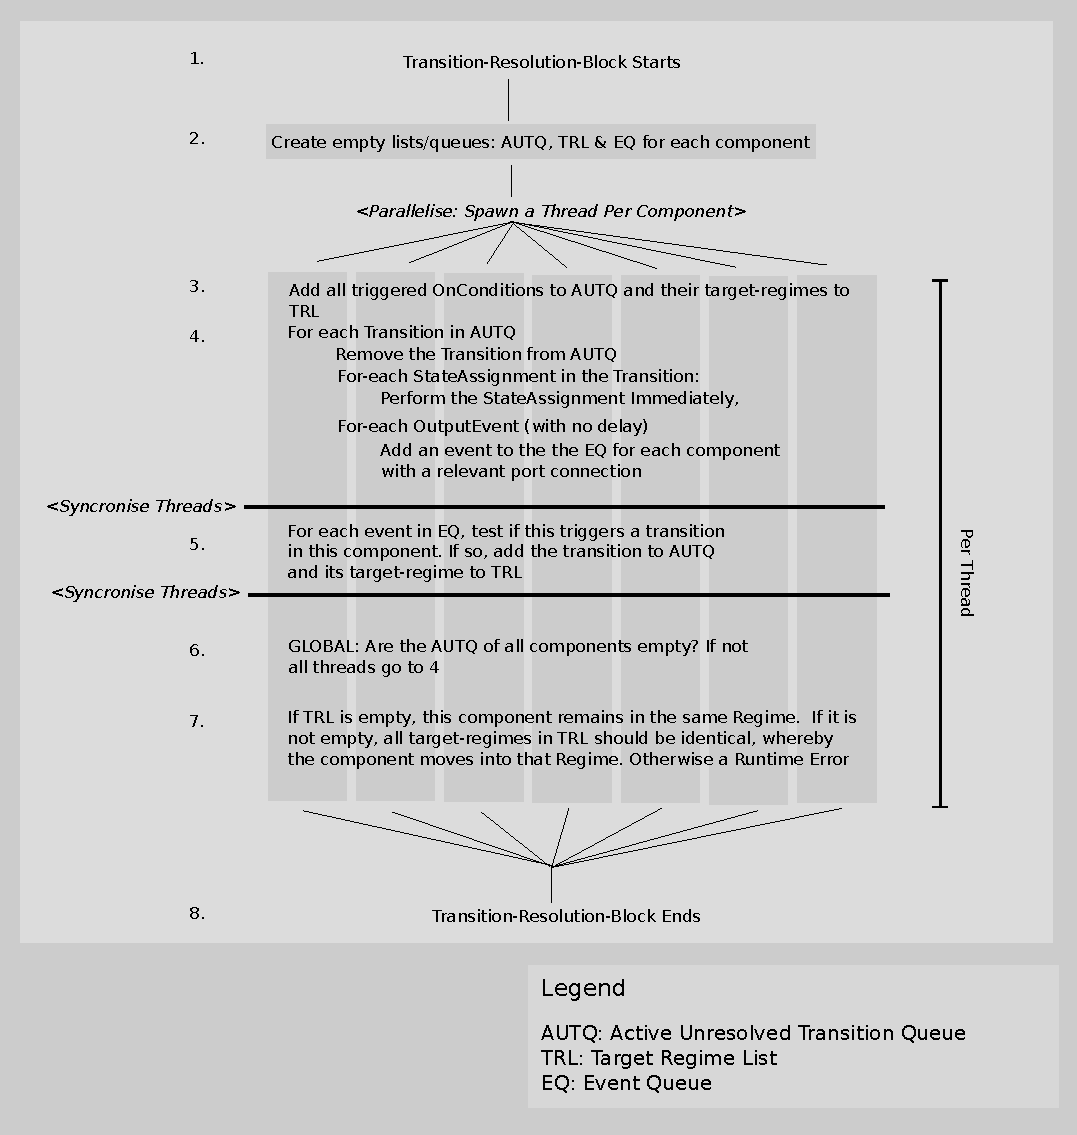
\includegraphics[width=14cm]{al/ParallelisingTransitions.pdf}example_IzRegimeTransGraph.pdf
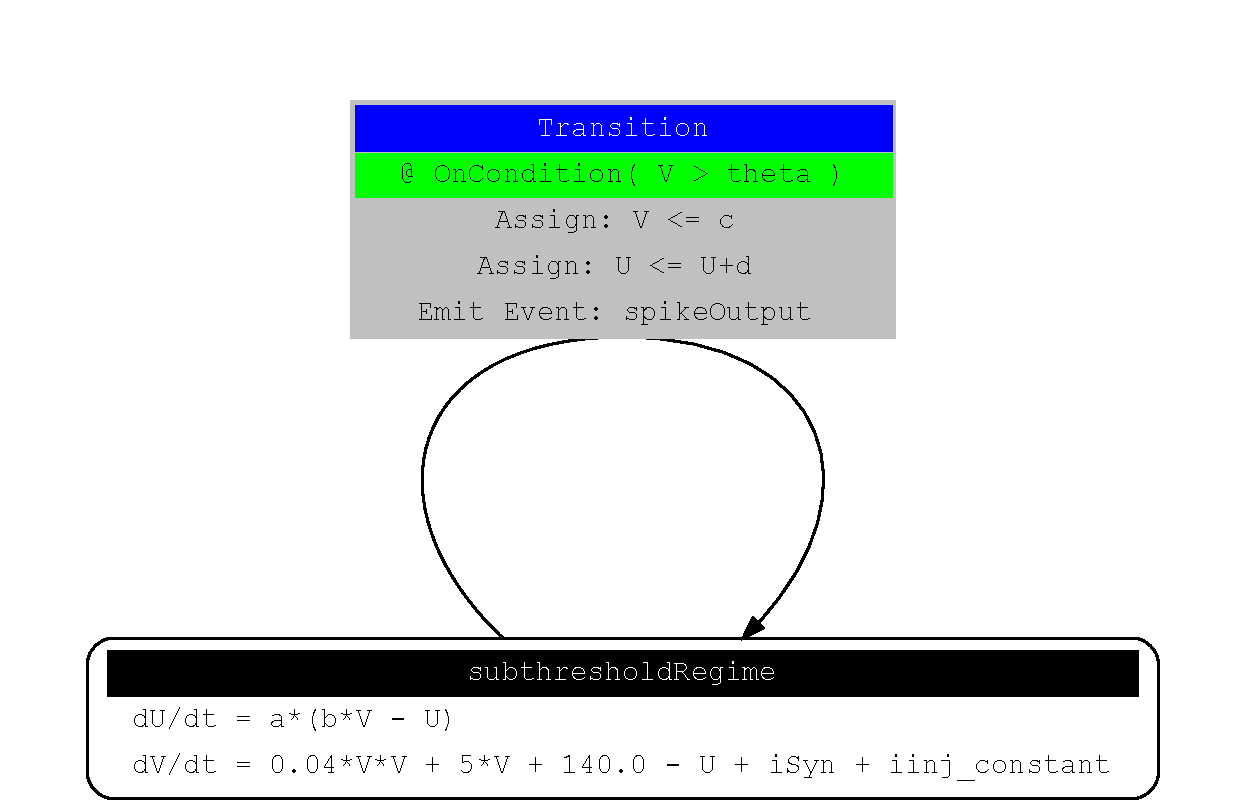
\includegraphics[width=8cm]{figures/example_IzRegimeTransGraph.pdf}
\protect\caption{{\tt RegimeGraph} for the XML model in this section.}
\label{fig:EX3_RegimeGraph}
\end{figure}

\noindent
Using this Abstraction Layer definition, as well as suitable parameters from the
user layer; $a=0.02, b=0.2, c=-65, d= 8, iinj\_constant= 5.0$, we can simulate
this, giving output as shown in Figure~\ref{fig:Ex1_Output}.

In Figure~\ref{fig:Ex1_Output}, we can see the value of the \StateVariable $V$
over time. We can also see that when the value of $V>theta$ triggers the
condition, we emit a spike, and the \StateAssignment of $V \leftarrow c$ resets
the value of $V$.
%
\noindent
The corresponding Abstraction Layer XML description for this model is the following:
%
\begin{lstlisting}

<?xml version='1.0' encoding='UTF-8'?>
<NineML xmlns="http://nineml.org/9ML/0.1">
    xmlns:xsi="http://www.w3.org/2001/XMLSchema-instance"
    xsi:schemaLocation="http://nineml.org/9ML/0.1 NineML\_v0.2.xsd">

  <ComponentClass name="izhikevichCellNew">

    <Parameter name="a" dimension="none"/>
    <Parameter name="c" dimension="voltage"/>
    <Parameter name="b" dimension="per_time"/>
    <Parameter name="d" dimension="voltage_per_time"/>
    <Parameter name="theta" dimension="voltage"/>

    <AnalogPort name="iSyn" mode="reduce" reduce_op="+" dimension="current"/>
    <AnalogPort name="U" mode="send" dimension="none"/>
    <AnalogPort name="V" mode="send" dimension="voltage"/>
    <EventPort name="spikeOutput" mode="send"/>


    <Dynamics>

        <StateVariable name="V" dimension="voltage"/>
        <StateVariable name="U" dimension="voltage_per_time"/>

        <Alias name="rv" dimension="none">
            <MathInline>V*U</MathInline>
        </Alias>

        <Regime name="subthresholdRegime">

          <TimeDerivative variable="U">
            <MathInline>a*(b*V - U)</MathInline>
          </TimeDerivative>

          <TimeDerivative variable="V">
            <MathInline>0.04*V*V + 5*V + 140.0 - U + iSyn</MathInline>
          </TimeDerivative>


          <OnCondition>
            <Trigger>
              <MathInline>V \&gt; theta </MathInline>
            </Trigger>

            <StateAssignment variable="V" >
              <MathInline>c</MathInline>
            </StateAssignment>

            <StateAssignment variable="U" >
              <MathInline>U+d</MathInline>
            </StateAssignment>

            <EventOut port="spikeOutput" />

          </OnCondition>

        </Regime>
    </Dynamics>

  </ComponentClass>
</NineML>
\end{lstlisting}

User Layer description for the above example:

\begin{lstlisting}
<?xml version='1.0' encoding='UTF-8'?>
<nineml xmlns="http://www.NineML.org/9ML/1.0" name="Izhikevich neuron">
  <import language="NineML">
    http://www.NineML.org/1.0/dimensions.9ml
  </import>
  <component name="Izhikevich neuron">
    <definition language="NineML">
      http://www.NineML.org/neurons/izhikevichCellNew.9ml
    </definition>
    <property name="V">
       <quantity>
         <value>
           <scalar>-60</scalar>
           <unit>mV</unit>
         </value>
       </quantity>
       <note><String>Initial value</String></note>
    </property>
    <property name="U">
       <quantity>
         <value>
           <scalar>0</scalar>
           <unit>mV_per_ms</unit>
         </value>
       </quantity>
       <note><String>Initial value</String></note>
    </property>
    <property name="theta">
       <quantity>
         <value>
           <scalar>50</scalar>
           <unit>mV</unit>
         </value>
       </quantity>
       <note><String>Parameter value (spike amplitude)</String></note>
    </property>
    <property name="a">
       <quantity>
         <value>
           <scalar>0.02</scalar>
           <unit>none</unit>
         </value>
       </quantity>
       <note><String>Parameter value</String></note>
    </property>
    <property name="b">
       <quantity>
         <value>
           <scalar>0.2</scalar>
           <unit>per_ms</unit>
         </value>
       </quantity>
       <note><String>Parameter value</String></note>
    </property>
    <property name="c">
       <quantity>
         <value>
           <scalar>-65</scalar>
           <unit>mV</unit>
         </value>
       </quantity>
       <note><String>Parameter value (reset voltage)</String></note>
    </property>
    <property name="d">
       <quantity>
         <value>
           <scalar>8</scalar>
           <unit>mV_per_ms</unit>
         </value>
       </quantity>
       <note><String>Parameter value</String></note>
    </property>
  </component>
</nineml>
\end{lstlisting}

Here, we show the simulation results of this XML representation.
\begin{figure}[htb!]
\center
%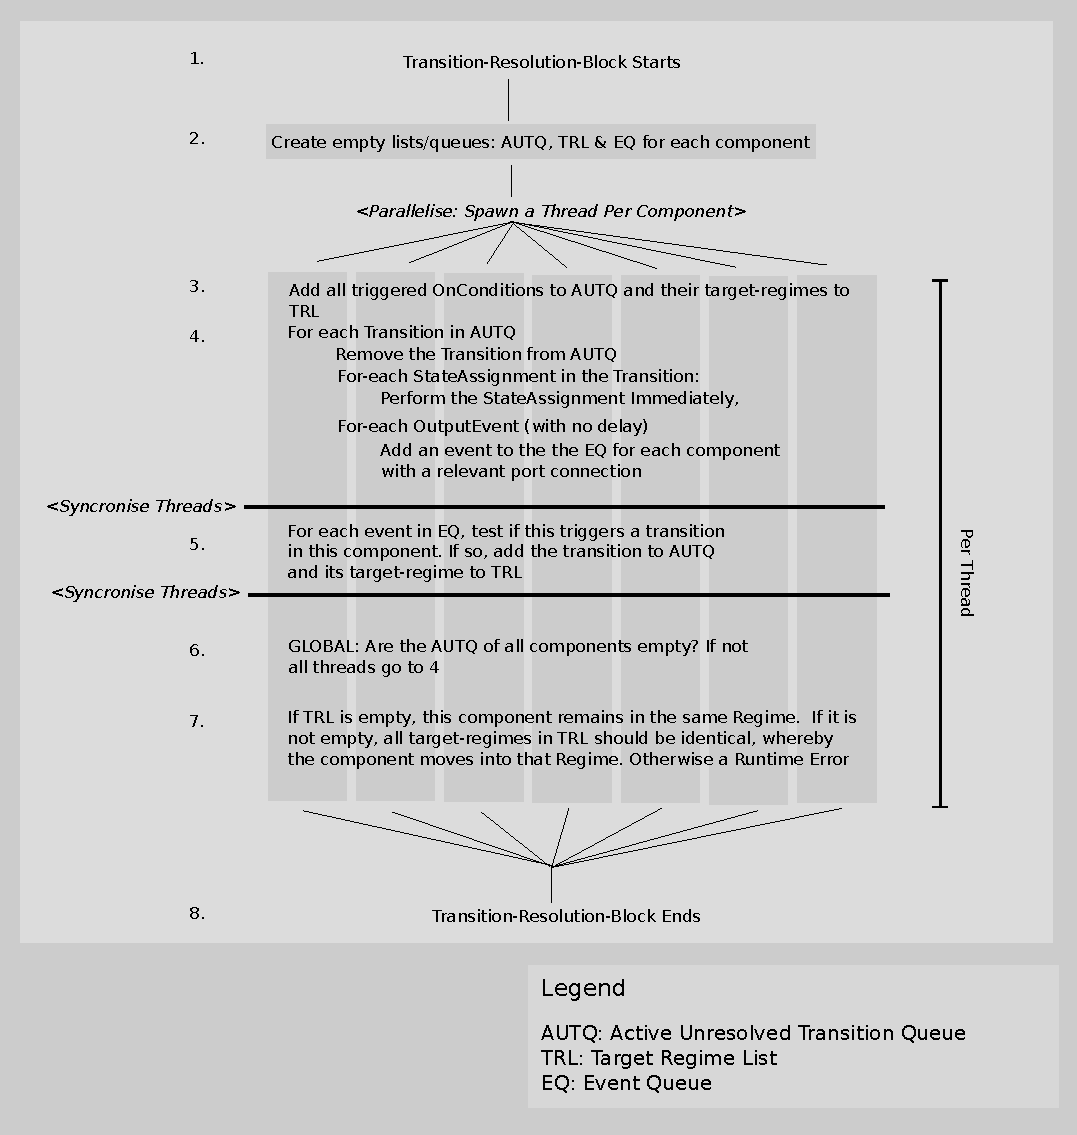
\includegraphics[width=14cm]{al/ParallelisingTransitions.pdf}example_IzRegimeTransGraph.pdf
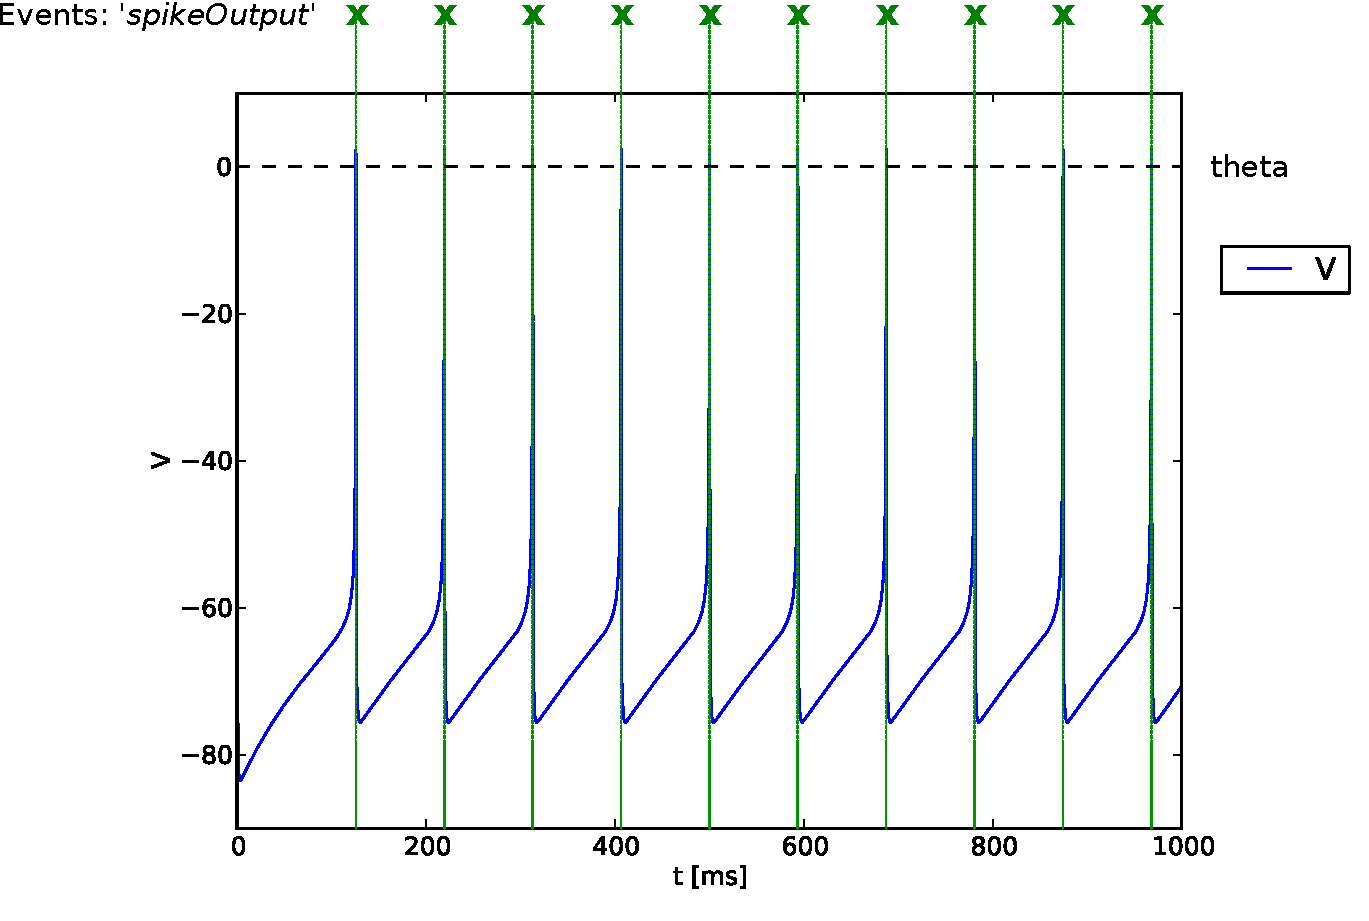
\includegraphics[width=8cm]{figures/example_IzVoltageWave.pdf}
\protect\caption{Result of simulating of the XML model in
this section}
\label{fig:Ex1_Output}
\end{figure}

\newpage
\subsection{Second XML example}

In this example, we build a representation of a integrate-and-fire neuron, with
an attached input synapse.
\noindent
We have a single \StateVariable, $iaf\_V$.
This time, the neuron has an absolute refractory period; which is implemented
by using 2 regimes. $RegularRegime$ \& $RefractoryRegime$
In $RegularRegime$, the neuron voltage evolves as:
\begin{eqnarray}
\frac{d(iaf\_V)}{dt} = \frac{ iaf\_gl*( iaf\_vrest - iaf\_V ) + iaf\_ISyn+cobaExcit\_I} {iaf\_cm}
\end{eqnarray}
In $RefractoryRegime$, the neuron voltage does not change in response to any
input:

\begin{eqnarray}
\frac{d(iaf\_V)}{dt} = 0
\end{eqnarray}
\noindent
In both Regimes, the synapses dynamics evolve as:
\begin{eqnarray}
\frac{d(cobaExcit\_g)}{dt} = - \frac{cobaExcit\_g}{cobaExcit\_tau}
\end{eqnarray}
\noindent
The neuron has 2 EventPorts, $iaf\_spikeoutput$ is a send port, which sends
events when the neuron fires, and $cobaExcit\_spikeinput$ is a recv port,
which tells the attached synapse that it should `fire'.
\noindent
The neuron has 4 {\Transition}s, 2 {\OnEvent}s  and 2 {\OnCondition}s.
Two of the Transitions are triggered by $cobaExcit\_spikeinput$ events, which
cause the conductance of the synapse to increase by an amount $q$, These
happen in both Regimes.
The other {\OnCondition}s:
\begin{itemize}
\item One is triggered the voltage being above threshold, which moves the
component from $RegularRegime$ to $RefractoryRegime$, sets V to the
reset-voltage also emits a spike
\item The other is triggered by enough time having passed for the component
to come out of the $RefractoryRegime$ and move back to the $RegularRegime$
\end{itemize}

The corresponding Regime Graph is shown in Figure 5.

\begin{figure}[htb!]
\center
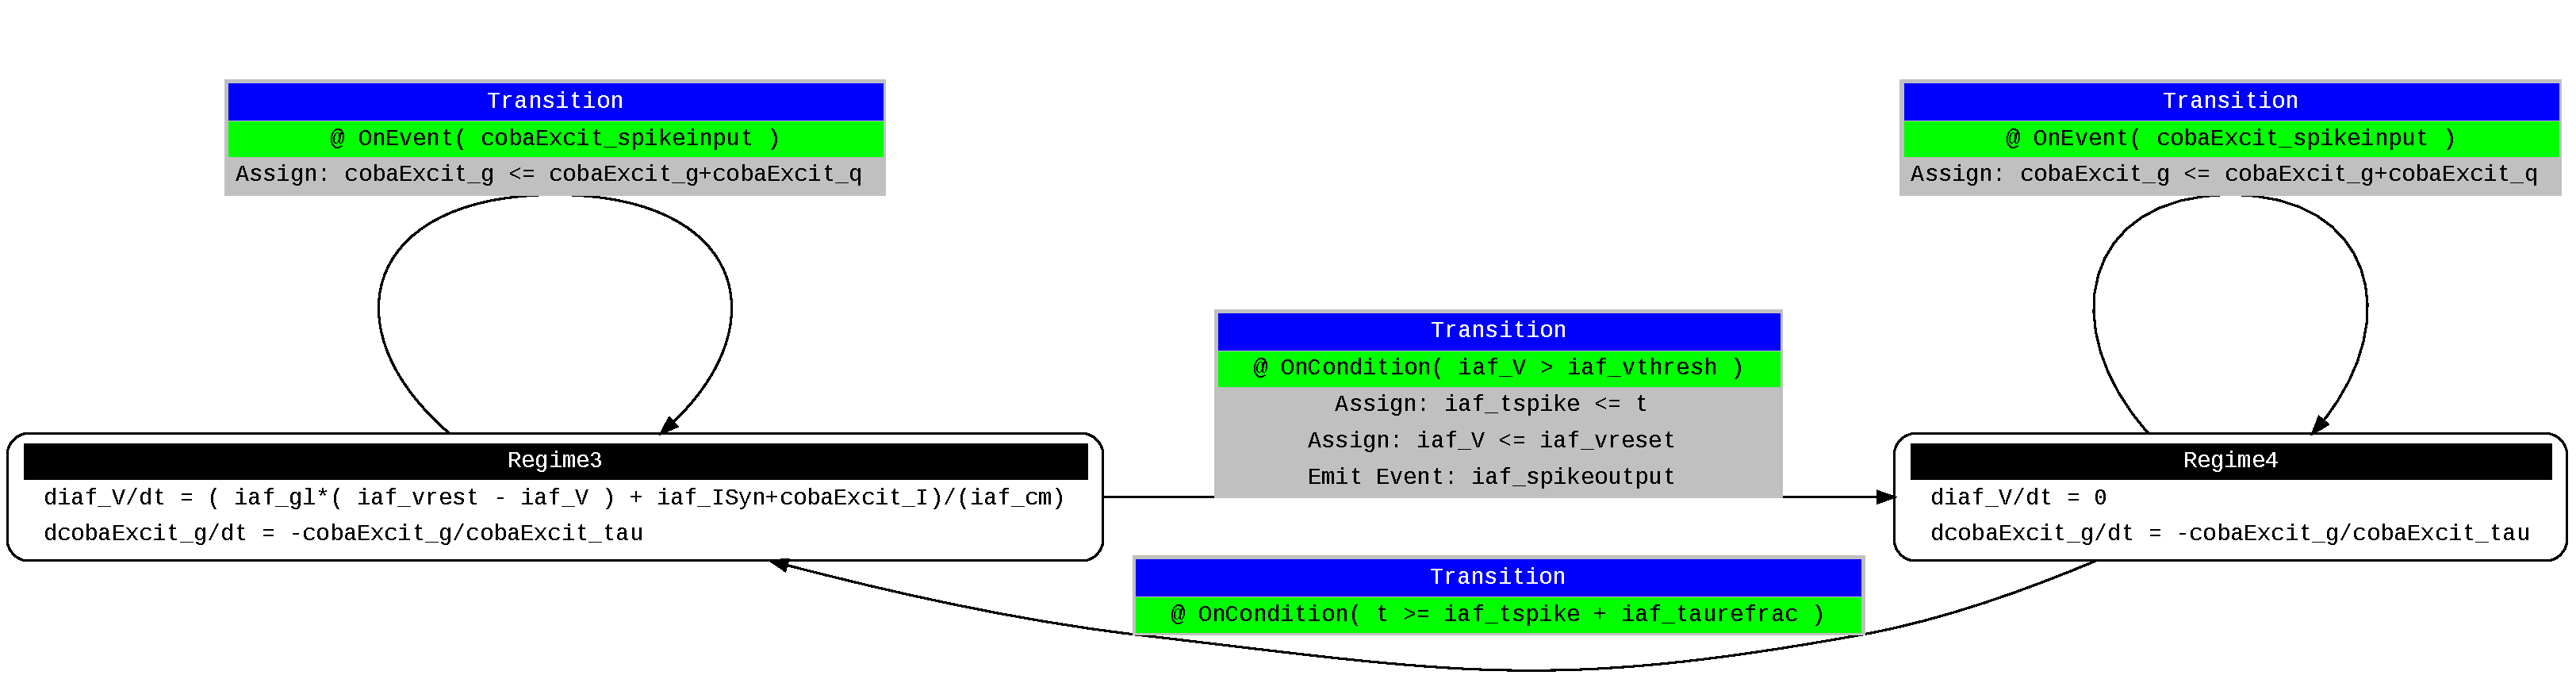
\includegraphics[width=14cm]{figures/demo2_Coba1_trnasition.pdf}
\protect\caption{RegimeGraph for the XML model in this section}
\label{fig:EX2_trans}
\end{figure}

The resulting XML description for the Abstraction Layer is :

\begin{lstlisting}[label=code:xmliaf2]
<?xml version='1.0' encoding='UTF-8'?>
<NineML xmlns="http://nineml.org/9ML/0.1">
  <ComponentClass name="iaf_1coba">
    <AnalogPort mode="send" name="iaf_V"/>
    <AnalogPort mode="reduce" reduce_op="+" name="iaf_ISyn"/>
    <AnalogPort mode="send" name="cobaExcit_I"/>
    <EventPort mode="send" name="iaf_spikeoutput"/>
    <EventPort mode="recv" name="cobaExcit_spikeinput"/>
    <Parameter dimension="area" name="iaf_cm"/>
    <Parameter dimension="time" name="iaf_taurefrac"/>
    <Parameter dimension="conductance" name="iaf_gl"/>
    <Parameter dimension="voltage" name="iaf_vreset"/>
    <Parameter dimension="voltage" name="iaf_vrest"/>
    <Parameter dimension="voltage" name="iaf_vthresh"/>
    <Parameter dimension="time" name="cobaExcit_tau"/>
    <Parameter dimension="conductance" name="cobaExcit_q"/>
    <Parameter dimension="voltage" name="cobaExcit_vrev"/>
    <Dynamics>
      <Regime name="RefractoryRegime">
        <TimeDerivative variable="iaf_V">
          <MathInline>0</MathInline>
        </TimeDerivative>
        <TimeDerivative variable="cobaExcit_g">
          <MathInline>-cobaExcit_g/cobaExcit_tau</MathInline>
        </TimeDerivative>
        <OnEvent target_regime="RefractoryRegime" src_port="cobaExcit_spikeinput">
          <StateAssignment variable="cobaExcit_g">
            <MathInline>cobaExcit_g+cobaExcit_q</MathInline>
          </StateAssignment>
        </OnEvent>
        <OnCondition target_regime="RegularRegime">
          <Trigger>
            <MathInline>t &gt;= iaf_tspike + iaf_taurefrac</MathInline>
          </Trigger>
        </OnCondition>
      </Regime>
      <Regime name="RegularRegime">
        <TimeDerivative variable="iaf_V">
          <MathInline>( iaf_gl*( iaf_vrest - iaf_V ) + iaf_ISyn+cobaExcit_I)/(iaf_cm)</MathInline>
        </TimeDerivative>
        <TimeDerivative variable="cobaExcit_g">
          <MathInline>-cobaExcit_g/cobaExcit_tau</MathInline>
        </TimeDerivative>
        <OnEvent target_regime="RegularRegime" src_port="cobaExcit_spikeinput">
          <StateAssignment variable="cobaExcit_g">
            <MathInline>cobaExcit_g+cobaExcit_q</MathInline>
          </StateAssignment>
        </OnEvent>
        <OnCondition target_regime="RefractoryRegime">
          <StateAssignment variable="iaf_tspike">
            <MathInline>t</MathInline>
          </StateAssignment>
          <StateAssignment variable="iaf_V">
            <MathInline>iaf_vreset</MathInline>
          </StateAssignment>
          <EventOut port="iaf_spikeoutput"/>
          <Trigger>
            <MathInline>iaf_V &gt; iaf_vthresh</MathInline>
          </Trigger>
        </OnCondition>
      </Regime>
      <Alias name="cobaExcit_I">
        <MathInline>cobaExcit_g*(cobaExcit_vrev-iaf_V)</MathInline>
      </Alias>
      <StateVariable dimension="voltage" name="iaf_V"/>
      <StateVariable dimension="time" name="iaf_tspike"/>
      <StateVariable dimension="conductance" name="cobaExcit_g"/>
    </Dynamics>
  </ComponentClass>
</NineML>

\end{lstlisting}

User Layer description for the above example:

\begin{lstlisting}
<?xml version='1.0' encoding='UTF-8'?>
<nineml xmlns="http://www.NineML.org/9ML/1.0" name="IaF neuron with synapse">
  <import language="NineML">
    http://www.NineML.org/1.0/dimensions.9ml
  </import>
  <component name="IaF neuron">
    <definition language="NineML">
      http://www.NineML.org/neurons/iaf_1coba.9ml
    </definition>
    <property name="iaf_V">
       <quantity>
         <value>
           <scalar>-60</scalar>
           <unit>mV</unit>
         </value>
       </quantity>
       <note><String>Initial value</String></note>
    </property>
    <property name="iaf_tspike">
       <quantity>
         <value>
           <scalar>-1</scalar>
           <unit>ms</unit>
         </value>
       </quantity>
       <note><String>Initial value</String></note>
    </property>
    <property name="cobaExcit_g">
       <quantity>
         <value>
           <scalar>0</scalar>
           <unit>mS</unit>
         </value>
       </quantity>
       <note><String>Initial value</String></note>
    </property>
    <property name="iaf_cm">
       <quantity>
         <value>
           <scalar>0.02</scalar>
           <unit>cm_square</unit>
         </value>
       </quantity>
       <note><String>Parameter value</String></note>
    </property>
    <property name="iaf_taurefrac">
       <quantity>
         <value>
           <scalar>3</scalar>
           <unit>ms</unit>
         </value>
       </quantity>
       <note><String>Parameter value (refractory period)</String></note>
    </property>
    <property name="iaf_gl">
       <quantity>
         <value>
           <scalar>0.1</scalar>
           <unit>mS</unit>
         </value>
       </quantity>
       <note><String>Parameter value (leak conductance)</String></note>
    </property>
    <property name="iaf_vreset">
       <quantity>
         <value>
           <scalar>-70</scalar>
           <unit>mV</unit>
         </value>
       </quantity>
       <note><String>Parameter value (reset voltage)</String></note>
    </property>
    <property name="iaf_vrest">
       <quantity>
         <value>
           <scalar>-60</scalar>
           <unit>mV</unit>
         </value>
       </quantity>
       <note><String>Parameter value (resting potential)</String></note>
    </property>
    <property name="iaf_vthresh">
       <quantity>
         <value>
           <scalar>20</scalar>
           <unit>mV</unit>
         </value>
       </quantity>
       <note><String>Parameter value (threshold potential)</String></note>
    </property>
    <property name="cobaExcit_tau">
       <quantity>
         <value>
           <scalar>2</scalar>
           <unit>ms</unit>
         </value>
       </quantity>
       <note><String>Parameter value (synaptic time constant)</String></note>
    </property>
    <property name="cobaExcit_q">
       <quantity>
         <value>
           <scalar>1</scalar>
           <unit>ms</unit>
         </value>
       </quantity>
       <note><String>Parameter value (conductance increase on spike)</String></note>
    </property>
    <property name="cobaExcit_vrev">
       <quantity>
         <value>
           <scalar>0</scalar>
           <unit>mV</unit>
         </value>
       </quantity>
       <note><String>Parameter value (synaptic reversal potential)</String></note>
    </property>
  </component>
</nineml>
\end{lstlisting}

The simulation results is presented in Figure 6.
\begin{figure}[htb!]
\center
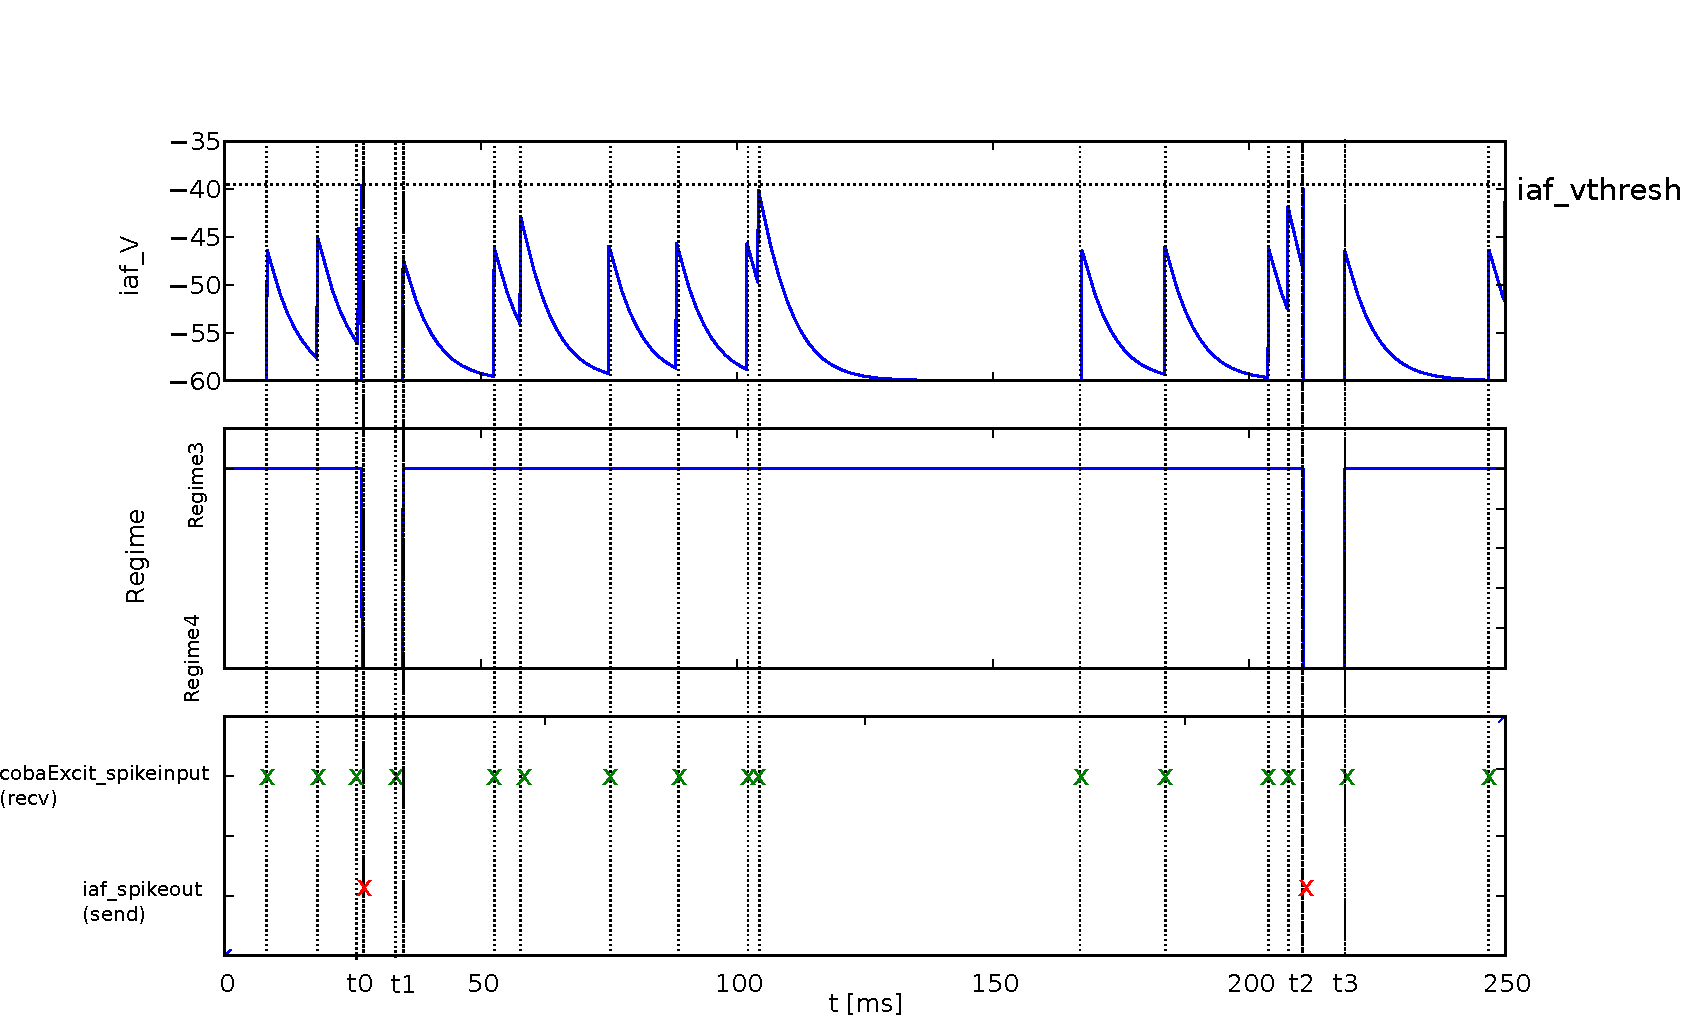
\includegraphics[width=14cm]{figures/demo2_Coba1_out.pdf}
\protect\caption{Result of simulating of the XML model in this section.
$cobaExcit\_spikeinput$ is fed events from an external Poisson generator
in this simulation}
\label{fig:EX2_Output}
\end{figure}

\pagebreak

\newpage

\section{Transition Resolution}
\label{resolution}

This section outlines pseudo code which defines the order of
\Transition-triggering, state assignment execution, event emission,
transmission and resolution in a system of connected components.
Implementations do not need to implement this algorithm but should produce
the same behaviours.

A {\tt TransitionResolutionBlock} represents an instant in time. It begins
before any {\Transition}s occur and ends after each component has moved
into its new \Regime, all \textbf{StateAssignments} have been executed
and all Events generated and resolved in the system.

\subsection{Serial Implementation of Transition Resolution}

\newcommand{\CN}[0]{\textsl{C\_n}}

We have a system of \textsl{N} components \textsl{\{C\_1,C\_2,...,C\_N\}},
at time, \textsl{t}, where each component, \CN, is in \Regime
$R^{t}_{n}$.

\noindent From \Regime $R^{t}_{n}$, there are:
\begin{itemize}
\item OnEvent {\Transition}s $OnEv^{t}_{n} = \{ ... \}$
\item OnCondition {\Transition}s $OnCond^{t}_{n} = \{ ... \}$
\end{itemize}

\newcommand{\send}[0]{\texttt{send} }
\newcommand{\recv}[0]{\texttt{recv} }

\noindent Component \CN
has:
\begin{itemize}
\item \send EventPorts \textsl{EvSend = \{$EvSend_{n,1,}$, $EvSend_{n,2,}$, ... \}}
\item \recv EventPorts \textsl{EvRecv = \{$EvRecv_{n,1,}$, $EvRecv_{n,2,}$, ... \}}
\end{itemize}

\noindent EventPort connections are stored in a a map,
\textsl{EvPortConnections}, which maps EvSend to a list of EvRecv ports. i.e.,

\textsl{\{EvSend $\rightarrow$ [EvRecv,EvRecv,..,EvRecv], EvSend $\rightarrow$
[EvRecv,EvRecv,EvRecv,...,EvRecv]\}}.

\newcommand{\RCLn}{$RCL_n$}
\newcommand{\AUTQn}{$AUTQ_n$}
\newcommand{\EQn}{$EQ_n$}

\noindent Each component has 3 associated data structures
\begin{itemize}
\item RegimeChangeList (\RCLn) (This list will contain target-regimes of
triggered transitions)
\item ActiveUnresolvedTransitionsQueue (\AUTQn) (This queue will
contain transitions which will occur, but their effects have not be
evaluated yet)
\item EventQueue (\EQn) (This list contains events delivered to this
component from other components via EventPort-connections)
\end{itemize}

\subsubsection{Algorithm}

\begin{enumerate}
\item Enter {\tt TransitionResolutionBlock}
\item For each component, \CN: clear \RCLn, \AUTQn and \EQn.
\item For each component, \CN: for each \textsl{oncond} in $OnCond^{t}_{n}$ : if
\textsl{oncond.trigger} evaluates to true, add \textsl{oncond} to \AUTQn.
\item For each component, \CN:  for each \textsl{tr} in \AUTQn :
\begin{itemize}
\item
remove \textsl{tr} from \AUTQn
\item add the target\_regime to \RCLn
\item for each
\textsl{action} in \textsl{tr.do}:
\begin{itemize}
\item if \textsl{action} is an OutputEvent: test
if the OutputEvent port is a key in \textsl{EvPortConnections}. If so, add the
    OutputEvent to the EventQueue (\textsl{EQ\_{target}}) corresponding to each
    \textsl{EvRecv} in the \textsl{EvPortConnections} map.

\item  if \textsl{action}  is a StateAssignment, execute that state-assignment
immediately.
\end{itemize}
\end{itemize}

\item For each component \CN: for each event, \textsl{EvRecv} in \EQn: test
whether there is a transition, \textsl{tr} triggered by this event, i.e an
OnEvent in $OnEv^t_n$ from $R^t_n$ ; if so; then add it to \AUTQn.

\item While any component has a non-empty \textsl{AUTQ}: Goto (4).

\item For each component, \CN, check that all the target-regimes in the \RCLn
are the same regime. (If not raise a RuntimeError). Each component moves into
this target-regime, or remains in the same regime if \RCLn is empty.

\item Leave {\tt TransitionResolutionBlock}

\end{enumerate}

\subsubsection{Notes}

\begin{enumerate}
\item  There is no order defined in transitions; this means
that the order of resolution of state assignments can be ambiguous. If, for
example, we have two transitions, T1 and T2, originating from the same \Regime,
in which T1 contains the state assignment \textsl{V=V+1} and T2 contains the
assignment \textsl{V=V*V}, and both transitions are triggered, then there is no
guarantee about the value of V. It is up the user to ensure this does not
happen.

\item This Resolution System allows \emph{cascading} of Events, which in theory
could be recursive through components, depending on connectivity. The
implementation allows for this; and it is the users responsibility to ensure
that there are not such issues. The implementation may decided to terminate
Step (6) after a given number (say 1000) of iterations to prevent infinite
loops.

\item Flattening of hierarchical components; implementation should ensure that
the behaviour of a flattened component is identical to that of an unflattened
component.
\end{enumerate}

\subsection{Parallelising of Event Resolution}

This algorithm can be parallelised as following. We create a thread for each
Component, which can independently execute Steps (3 to 6). The threads need
to be synchronized after steps (4) and (5) as shown in
Figure~\ref{ParallelisingTransitions}.


\section{Acknowledgments}

%This work was made possible by grant R01 GM070923 from the NIH National
%Institute of General Medical Sciences (USA) for continued development and
%support of SBML and related software infrastructure.


\clearpage
\bibliography{sbmlpkgspec}



% -----------------------------------------------------------------------------
% End of document
% -----------------------------------------------------------------------------

\end{document}
